%=======================================================================
%  BTP Phase 1 -- Review 1
%  Graph-Theoretic Register Allocation in an SSA-Based Compiler Backend
%
%  ENGINE: XeLaTeX  (Overleaf: Menu -> Compiler -> XeLaTeX)
%  ASSETS: iiitk-logo.jpeg  (optional -- deck compiles without it)
%
%  Two outputs from this one file:
%    xelatex btp-review1.tex                      -> clean deck
%    xelatex "\def\SHOWNOTES{}%=======================================================================
%  BTP Phase 1 -- Review 1
%  Graph-Theoretic Register Allocation in an SSA-Based Compiler Backend
%
%  ENGINE: XeLaTeX  (Overleaf: Menu -> Compiler -> XeLaTeX)
%  ASSETS: iiitk-logo.jpeg  (optional -- deck compiles without it)
%
%  Two outputs from this one file:
%    xelatex btp-review1.tex                      -> clean deck
%    xelatex "\def\SHOWNOTES{}%=======================================================================
%  BTP Phase 1 -- Review 1
%  Graph-Theoretic Register Allocation in an SSA-Based Compiler Backend
%
%  ENGINE: XeLaTeX  (Overleaf: Menu -> Compiler -> XeLaTeX)
%  ASSETS: iiitk-logo.jpeg  (optional -- deck compiles without it)
%
%  Two outputs from this one file:
%    xelatex btp-review1.tex                      -> clean deck
%    xelatex "\def\SHOWNOTES{}%=======================================================================
%  BTP Phase 1 -- Review 1
%  Graph-Theoretic Register Allocation in an SSA-Based Compiler Backend
%
%  ENGINE: XeLaTeX  (Overleaf: Menu -> Compiler -> XeLaTeX)
%  ASSETS: iiitk-logo.jpeg  (optional -- deck compiles without it)
%
%  Two outputs from this one file:
%    xelatex btp-review1.tex                      -> clean deck
%    xelatex "\def\SHOWNOTES{}\input{btp-review1}" -> deck + speaker notes
%=======================================================================
\documentclass[aspectratio=169,11pt]{beamer}

\usepackage{fontspec}
% Carlito = metric clone of Calibri (the template's font).
% Resolved by family name (works locally via fontconfig) or by filename
% (works on Overleaf via the TeX Live tree). Warns loudly if neither works,
% rather than silently falling back to a font that isn't the template's.
\IfFontExistsTF{Carlito}{%
  \setsansfont{Carlito}%
}{%
  \IfFontExistsTF{Carlito-Regular.ttf}{%
    \setsansfont{Carlito}[Extension=.ttf,UprightFont=*-Regular,
      BoldFont=*-Bold,ItalicFont=*-Italic,BoldItalicFont=*-BoldItalic]%
  }{%
    \GenericWarning{}{** CARLITO NOT FOUND -- deck will not match the
      institute template. Install/enable the carlito font. **}%
  }%
}
\usepackage{booktabs}
\usepackage{adjustbox}
\usepackage{graphicx}
\usepackage{xcolor}
\usepackage{tikz}
\usetikzlibrary{arrows.meta,positioning,fit,backgrounds,calc,shapes.geometric}

%----------------------------------------------------------------------
% 1. COLOURS  (from the institute template's Office theme)
%----------------------------------------------------------------------
\definecolor{iiitkblue}{HTML}{4472C4}   % template accent1
\definecolor{iiitkdark}{HTML}{44546A}   % template dk2
\definecolor{regA}{HTML}{4472C4}
\definecolor{regB}{HTML}{ED7D31}
\definecolor{regC}{HTML}{70AD47}
\definecolor{lyrIn}{HTML}{E8EEF9}
\definecolor{lyrAna}{HTML}{E7F0E3}
\definecolor{lyrAlloc}{HTML}{FBE9DC}
\definecolor{lyrBack}{HTML}{EFEAF4}
\definecolor{lyrEval}{HTML}{FDF3D8}

%----------------------------------------------------------------------
% 2. THEME  (matches BTP Presentation Template-2-2.pptx)
%    white ground, black left-aligned titles, logo top-right,
%    centred institute footer, frame number bottom-right
%----------------------------------------------------------------------
\usetheme{default}
\setbeamercolor{normal text}{fg=black,bg=white}
\setbeamercolor{structure}{fg=iiitkblue}
\setbeamercolor{frametitle}{fg=black,bg=}
\setbeamercolor{itemize item}{fg=iiitkblue}
\setbeamercolor{itemize subitem}{fg=iiitkblue}
\setbeamertemplate{navigation symbols}{}
\setbeamertemplate{itemize item}{\raisebox{0.15ex}{\tiny$\bullet$}}
\setbeamertemplate{itemize subitem}{\raisebox{0.15ex}{\tiny$\circ$}}
\setbeamerfont{frametitle}{size=\large}
\setbeamerfont{framesubtitle}{size=\footnotesize}

% margins taken from the template master (1.10 cm at 16 cm slide width)
\setbeamersize{text margin left=1.1cm,text margin right=1.1cm}

% -- logo, placed at the template's exact coordinates, on every slide ---
\newcommand{\iiitklogo}{%
  \IfFileExists{iiitk-logo.jpeg}{\includegraphics[width=2.30cm]{iiitk-logo.jpeg}}{}}
\setbeamertemplate{background}{%
  \begin{tikzpicture}[overlay]
    \useasboundingbox (0,0) rectangle (\paperwidth,-\paperheight);
    \node[anchor=north east,inner sep=0pt]
      at ($(\paperwidth,0)+(-0.55cm,-0.10cm)$) {\iiitklogo};
  \end{tikzpicture}}

% -- frame title: black, left aligned, thin accent rule --------------
%    (delete the \rule line below for a pixel-plain template match)
\makeatletter
\setbeamertemplate{frametitle}{%
  \vspace{0.55cm}%
  \begin{minipage}{0.80\paperwidth}
    \raggedright\usebeamerfont{frametitle}\usebeamercolor[fg]{frametitle}%
    \insertframetitle\par
    \ifx\insertframesubtitle\@empty\else
      {\usebeamerfont{framesubtitle}\color{black!62}\insertframesubtitle\par}\fi
    \vspace{0.6mm}{\color{iiitkblue}\rule{\linewidth}{0.7pt}}
  \end{minipage}%
  \vspace{-0.15cm}}
\makeatother

\setbeamertemplate{footline}{%
  \hbox to \paperwidth{%
    \hspace*{1.1cm}%
    \hfill{\color{black!55}\fontsize{5.7}{7}\selectfont
           Indian Institute of Information Technology Kottayam}\hfill
    {\color{black!55}\fontsize{5.7}{7}\selectfont\insertframenumber}%
    \hspace*{1.1cm}}%
  \vspace{1.6mm}}

%----------------------------------------------------------------------
% 4. FIGURE 1 -- Slide 3: C code -> SSA with phi -> interference graph
%----------------------------------------------------------------------
\newcommand{\FigChordality}{%
\begin{adjustbox}{max width=\textwidth,max totalheight=3.1cm}
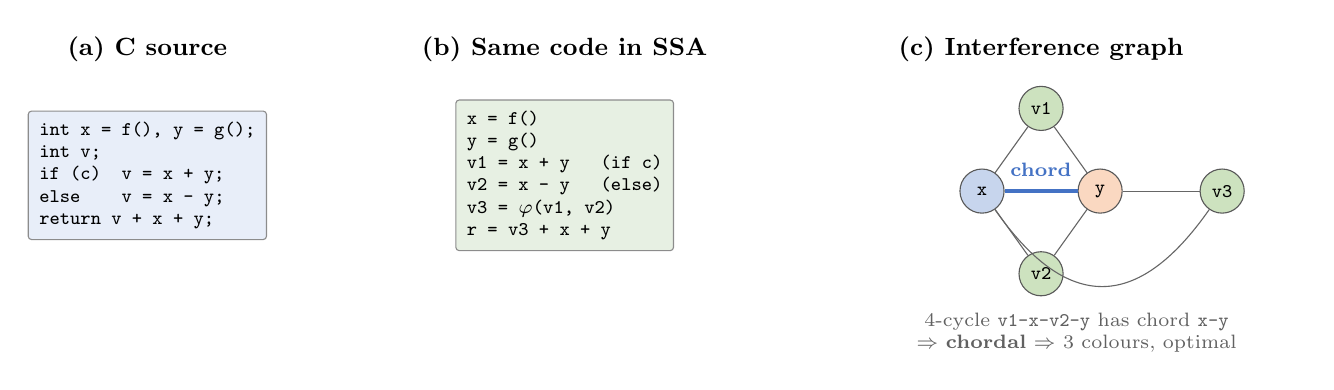
\begin{tikzpicture}[
  code/.style={draw=black!45,rounded corners=1.2pt,fill=lyrIn,align=left,
               inner sep=4pt,font=\scriptsize\ttfamily},
  ig/.style={draw=black!65,circle,inner sep=0pt,minimum size=0.56cm,font=\scriptsize},
  ed/.style={draw=black!60,thin},
  pcap/.style={font=\small\bfseries,align=center},
  ann/.style={font=\scriptsize,color=black!62,align=center}]

%---------------- (a) original C ----------------
\node[pcap] at (0,2.15) {(a) C source};
\node[code] (c1) at (0,0.55)
  {int x = f(), y = g();\\
   int v;\\
   if (c)\ \ v = x + y;\\
   else\ \ \ \ v = x - y;\\
   return v + x + y;};

%---------------- (b) SSA form ----------------
\begin{scope}[xshift=5.3cm]
  \node[pcap] at (0,2.15) {(b) Same code in SSA};
  \node[code,fill=lyrAna] (c2) at (0,0.55)
    {x\ = f()\\
     y\ = g()\\
     v1 = x + y\ \ \ (if c)\\
     v2 = x - y\ \ \ (else)\\
     v3 = $\varphi$(v1, v2)\\
     r\ = v3 + x + y};
\end{scope}

%---------------- (c) interference graph ----------------
\begin{scope}[xshift=10.6cm,yshift=0.35cm]
  \node[pcap] at (0.75,1.80) {(c) Interference graph};
  \node[ig,fill=regA!30] (vx)  at (0,0)        {\texttt{x}};
  \node[ig,fill=regB!30] (vy)  at (1.50,0)     {\texttt{y}};
  \node[ig,fill=regC!35] (v1)  at (0.75,1.05)  {\texttt{v1}};
  \node[ig,fill=regC!35] (v2)  at (0.75,-1.05) {\texttt{v2}};
  \node[ig,fill=regC!35] (v3)  at (3.05,0)     {\texttt{v3}};
  \draw[ed] (vx)--(v1); \draw[ed] (v1)--(vy);
  \draw[ed] (vx)--(v2); \draw[ed] (v2)--(vy);
  \draw[ed] (vy)--(v3);
  \draw[ed] (vx) to[out=-55,in=235,looseness=1.5] (v3);
  \draw[iiitkblue,line width=1.2pt] (vx)--(vy)
        node[midway,above=0.5mm,font=\scriptsize\bfseries,color=iiitkblue]{chord};
  \node[ann,text width=5.6cm] at (1.2,-1.80)
    {4-cycle \texttt{v1-x-v2-y} has chord \texttt{x-y} $\Rightarrow$
     \textbf{chordal} $\Rightarrow$ 3 colours, optimal};
\end{scope}
\end{tikzpicture}
\end{adjustbox}}

%----------------------------------------------------------------------
% 5. FIGURE 2 -- Slide 8: system pipeline, allocator is the swappable box
%----------------------------------------------------------------------
\newcommand{\FigPipeline}{%
\begin{adjustbox}{max width=\textwidth,max totalheight=6.0cm}
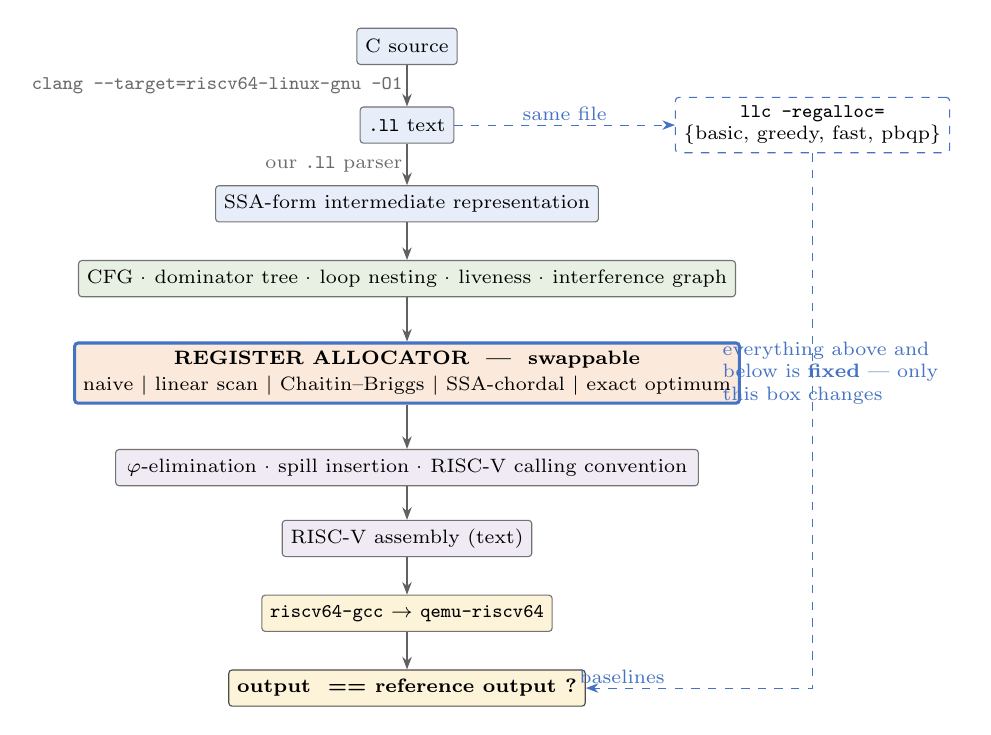
\begin{tikzpicture}[
  n/.style={draw=black!55,rounded corners=1.2pt,align=center,
            font=\scriptsize,inner sep=3pt,minimum height=0.46cm},
  wide/.style={n,minimum width=7.4cm},
  fl/.style={-{Stealth[length=1.6mm]},draw=black!62},
  lbl/.style={font=\scriptsize,color=black!58,inner sep=1.5pt}]

\node[n,fill=lyrIn]   (csrc) at (0, 0.00) {C source};
\node[n,fill=lyrIn]   (llt)  at (0,-1.00) {\texttt{.ll} text};
\node[n,fill=lyrIn]   (ir)   at (0,-2.00) {SSA-form intermediate representation};
\node[wide,fill=lyrAna] (ana) at (0,-2.95)
  {CFG \textperiodcentered\ dominator tree \textperiodcentered\ loop nesting
   \textperiodcentered\ liveness \textperiodcentered\ interference graph};
\node[wide,fill=lyrAlloc,draw=iiitkblue,line width=1.1pt] (alloc) at (0,-4.15)
  {\textbf{REGISTER ALLOCATOR \ --- \ swappable}\\[0.4mm]
   naive \textbar\ linear scan \textbar\ Chaitin--Briggs \textbar\
   SSA-chordal \textbar\ exact optimum};
\node[wide,fill=lyrBack] (back) at (0,-5.35)
  {$\varphi$-elimination \textperiodcentered\ spill insertion
   \textperiodcentered\ RISC-V calling convention};
\node[n,fill=lyrBack] (asm)  at (0,-6.25) {RISC-V assembly (text)};
\node[n,fill=lyrEval] (run)  at (0,-7.20)
  {\texttt{riscv64-gcc} $\rightarrow$ \texttt{qemu-riscv64}};
\node[n,fill=lyrEval,draw=black!70] (chk) at (0,-8.15)
  {\textbf{output \ ==\ reference output ?}};

\draw[fl] (csrc) -- node[lbl,left]{\texttt{clang --target=riscv64-linux-gnu -O1}} (llt);
\draw[fl] (llt)  -- node[lbl,left]{our \texttt{.ll} parser} (ir);
\draw[fl] (ir) -- (ana);
\draw[fl] (ana) -- (alloc);
\draw[fl] (alloc) -- (back);
\draw[fl] (back) -- (asm);
\draw[fl] (asm) -- (run);
\draw[fl] (run) -- (chk);

% fixed above and below: only the boxed allocator changes
\node[lbl,anchor=west,text width=3.0cm,align=left,color=iiitkblue]
     at (3.95,-4.15) {everything above and below is \textbf{fixed} --- only this box changes};

% external baselines off the same .ll
\node[n,fill=white,draw=regA,dashed,align=center] (llc) at (5.15,-1.00)
  {\texttt{llc -regalloc=}\\\{basic, greedy, fast, pbqp\}};
\draw[fl,draw=regA,dashed] (llt) -- node[lbl,above,color=regA]{same file} (llc);
\draw[fl,draw=regA,dashed] (llc) |- node[lbl,pos=0.92,above,color=regA]{baselines} (chk.east);
\end{tikzpicture}
\end{adjustbox}}

%======================================================================
\title{Design and Implementation of an SSA-Based RISC-V Compiler with
       Comparative Register Allocation}
\author{Shaun Alan Joseph \and Rishi Sharma \and Komal \and Aswin Parames}
\institute{Indian Institute of Information Technology Kottayam}
\date{9 September 2026}

\begin{document}

%======================= 1. TITLE =====================================
\begin{frame}
\vspace{0.9cm}
\begin{center}
{\large\textbf{Design and Implementation of an SSA-Based RISC-V Compiler\\[1mm]
 with Comparative Register Allocation}}\\[7mm]
{\footnotesize
\begin{tabular}{@{}c@{\hspace{7mm}}c@{\hspace{7mm}}c@{\hspace{7mm}}c@{}}
Shaun Alan Joseph & Rishi Sharma & Komal & Aswin Parames \\[0.4mm]
{\scriptsize\color{black!60}2023BCD0006} &
{\scriptsize\color{black!60}2023BCD0023} &
{\scriptsize\color{black!60}2023BCD0011} &
{\scriptsize\color{black!60}2023BCD0024} \\
\end{tabular}}\\[4mm]
{\footnotesize\textbf{Guided by:} Dr.\ Nandini J Warrier}\\[2mm]
{\footnotesize Dept.\ of Computer Science and Engineering}\\[1mm]
{\footnotesize Indian Institute of Information Technology, Kottayam}\\[5mm]
{\scriptsize\color{black!55} B.Tech Project \textperiodcentered\ Phase 1
 \textperiodcentered\ Review 1 \textperiodcentered\ 9 September 2026}
\end{center}
\end{frame}

%======================= 2. INTRODUCTION ==============================
\begin{frame}{Introduction: Register Allocation}
\textbf{The last big decision a compiler makes}
\begin{itemize}\small
  \item A program uses unlimited named values. A CPU has few \textbf{registers}
        --- 32 on RISC-V, 16 on x86-64
  \item Values that don't fit are \textbf{spilled} to memory. A spilled value
        costs a load and a store on \emph{every} access --- inside a loop,
        every iteration
  \item One of the highest-impact passes in a compiler backend
  \item \textbf{Chaitin (1981):} build an \textbf{interference graph} --- one
        node per value, an edge between values alive at the same time --- then
        colour it with \emph{k} colours, where \emph{k} = number of registers
\end{itemize}
\end{frame}

%======================= 3. SSA BACKGROUND ============================
\begin{frame}{Background: SSA Form}
\vspace{-1mm}
\begin{columns}[T]
\begin{column}{0.49\textwidth}
{\small\textbf{Static Single Assignment (SSA)}}
\begin{itemize}\scriptsize
  \item Every value assigned \textbf{exactly once}. Reassignment creates a new
        value: \texttt{x1}, \texttt{x2}, \texttt{x3}
  \item Where control flow merges, a \textbf{$\varphi$-function} picks whichever
        value arrived: \texttt{x3 = $\varphi$(x1, x2)}
  \item Used by LLVM, GCC, HotSpot, V8 --- the normal form of modern compilers
\end{itemize}
\end{column}
\begin{column}{0.49\textwidth}
{\small\textbf{Why SSA changes the problem}}
\begin{itemize}\scriptsize
  \item In general interference graphs can be \emph{any} shape, and colouring
        an arbitrary graph is NP-hard --- the textbook reason for heuristics
  \item Interference graphs of SSA programs are always \textbf{chordal}
  \item Chordal graphs colour \textbf{optimally, in linear time}
  \item Established by Hack \& Goos and by Pereira \& Palsberg, both 2005
\end{itemize}
\end{column}
\end{columns}
\vspace{2mm}
\centering\FigChordality
\end{frame}

%======================= 4a. LITERATURE (lines) =======================
\begin{frame}{Literature Survey}
\framesubtitle{Two lines of work}
\vspace{-1mm}
{\footnotesize\textbf{The classical line --- all heuristics, no optimality guarantee}}\par\vspace{1mm}
{\scriptsize
\begin{tabular}{@{}p{3.6cm}p{1.1cm}p{8.2cm}@{}}
\toprule
Work & Year & Contribution \\
\midrule
Chaitin et al.              & 1981 & Interference-graph formulation; showed the problem is NP-hard in general \\
Briggs, Cooper \& Torczon   & 1994 & \textbf{Optimistic colouring.} Ancestor of most production allocators \\
George \& Appel             & 1996 & Iterated coalescing --- removes redundant copy instructions \\
Poletto \& Sarkar           & 1999 & \textbf{Linear scan.} Drops graph colouring for speed; what JITs ship \\
\bottomrule
\end{tabular}}\par\vspace{2.5mm}
{\footnotesize\textbf{The SSA line --- and what it already established}}\par\vspace{1mm}
{\scriptsize
\begin{tabular}{@{}p{3.6cm}p{1.1cm}p{8.2cm}@{}}
\toprule
Work & Year & Contribution \\
\midrule
Tarjan \& Yannakakis          & 1984    & Linear-time chordality test and colouring order \\
\textbf{Hack \& Goos}         & 2005--06& SSA interference graphs are \textbf{chordal} $\Rightarrow$ optimal colouring in linear time \\
\textbf{Pereira \& Palsberg}  & 2005    & Built a chordal allocator, measured 23,681 Java methods. \textbf{$\sim$95\% of graphs are chordal} \\
Bouchez, Darte \& Rastello    & 2006    & The remaining hardness is in \textbf{spilling and coalescing}, not colouring \\
\bottomrule
\end{tabular}}
\end{frame}

%======================= 4b. LITERATURE (their numbers) ===============
\begin{frame}{Literature Survey}
\framesubtitle{Their measured results --- we reproduce these, we don't discover them}
\vspace{2mm}
\centering
{\footnotesize
\begin{tabular}{@{}p{5.4cm}p{7.4cm}@{}}
\toprule
Question & Published answer \emph{(Pereira \& Palsberg, Table 1)} \\
\midrule
Optimal vs.\ classical heuristic?          & \textbf{4.13 vs 4.17} registers/method --- under 1\% \\
Does $\varphi$-elimination destroy chordality? & \textbf{No --- it improves it.} 91\% $\rightarrow$ 95.5\% \\
Does the advantage survive few registers?  & Better at \emph{k}=6, roughly equal at \emph{k}=18 \\
\bottomrule
\end{tabular}}
\vspace{5mm}

\begin{minipage}{0.86\textwidth}\small
\textbf{We are not claiming to discover any of this.} These are the numbers we
expect to reproduce --- on a different processor, in our own compiler --- and
knowing them in advance is how we will tell whether our implementation is
correct.
\end{minipage}
\end{frame}

%======================= 5. MOTIVATION ================================
\begin{frame}{Motivation: Why Build Another One}
{\small\textbf{The algorithms are known. The comparison between them is not reliable.}}\par\vspace{2mm}
{\scriptsize Every published comparison used a different compiler, target and
benchmark set:}\par\vspace{1.5mm}
\centering
{\scriptsize
\begin{tabular}{@{}p{3.4cm}p{2.2cm}p{2.6cm}p{4.0cm}@{}}
\toprule
Work & Compiler & Target & Benchmarks \\
\midrule
Pereira \& Palsberg & JoeQ      & Java bytecode & Java standard library \\
Hack \& Goos        & libFirm   & x86           & SPEC \\
Poletto \& Sarkar   & their own & x86           & their own set \\
LLVM \texttt{greedy}& LLVM      & many          & LLVM's own suite \\
\bottomrule
\end{tabular}}\par\vspace{3mm}
\begin{minipage}{0.92\textwidth}\scriptsize
\textbf{So the numbers can't be placed side by side.} A difference between two
published results might be the algorithm --- or the compiler, the processor, or
the test programs.
\end{minipage}\par\vspace{2.5mm}
\begin{minipage}{0.92\textwidth}
{\small\textbf{What we build instead}}
\begin{itemize}\scriptsize
  \item \textbf{One} compiler, \textbf{one} IR, \textbf{one} benchmark set,
        \textbf{one} backend --- with the allocator as a swappable part
  \item Every difference in output is then caused by the algorithm and nothing else
  \item On \textbf{RISC-V}, where this comparison hasn't been published
\end{itemize}
\end{minipage}
\end{frame}

%======================= 6. PROBLEM STATEMENT =========================
\begin{frame}{Problem Statement}
\vspace{1mm}
\begin{minipage}{0.95\textwidth}
\small\textbf{Design and implement an SSA-based RISC-V compiler in which the
register allocator is a swappable component, implement five allocation
strategies, and compare them under identical conditions.}
\end{minipage}
\vspace{4mm}

{\small\textbf{Three things we measure}}
\begin{itemize}\small
  \item[\textbf{1}] \textbf{Allocation quality.} How many spills does each
        algorithm produce on the same program? Compared against LLVM's
        production allocators, and against a true optimum from an exact solver
        on small functions.
  \item[\textbf{2}] \textbf{Effect of register count.} RISC-V has two official
        integer register configurations --- \textbf{RV32I/RV64I with 32}, and
        \textbf{RV32E with 16}, used in embedded chips. We run every allocator
        on both. Real hardware, not an artificial setting.
  \item[\textbf{3}] \textbf{Cost of the algorithm.} How much work each allocator
        does, counted in operations rather than seconds, so the numbers
        reproduce on any machine.
\end{itemize}
\end{frame}

%======================= 7. SCOPE =====================================
\begin{frame}{Scope of Work}
\vspace{3mm}
\centering
{\footnotesize
\begin{tabular}{@{}p{2.1cm}p{10.6cm}@{}}
\toprule
Layer & Components \\
\midrule
Input      & Textual LLVM IR (\texttt{.ll}) parser, defined subset \\[0.8mm]
Analysis   & CFG \textperiodcentered\ dominator tree \textperiodcentered\ loop detection \textperiodcentered\ liveness \textperiodcentered\ interference graph \textperiodcentered\ chordality test \\[0.8mm]
Allocation & \textbf{Five allocators:} naive \textperiodcentered\ linear scan \textperiodcentered\ Chaitin--Briggs \textperiodcentered\ SSA/chordal \textperiodcentered\ exact optimum \textperiodcentered\ plus coalescing \\[0.8mm]
Backend    & $\varphi$-elimination \textperiodcentered\ spill insertion \textperiodcentered\ RISC-V calling convention \textperiodcentered\ assembly emission \\[0.8mm]
Validation & Static allocation verifier \textperiodcentered\ differential testing \textperiodcentered\ random program testing \\[0.8mm]
Evaluation & Metrics \textperiodcentered\ LLVM \texttt{llc} baselines \textperiodcentered\ 16- vs 32-register comparison \textperiodcentered\ plots \textperiodcentered\ graph visualiser \\
\bottomrule
\end{tabular}}
\vspace{5mm}

\begin{minipage}{0.93\textwidth}\footnotesize
\textbf{Beating LLVM's \texttt{greedy} is not a goal.} Landing within a
constant factor and explaining the gap is.
\end{minipage}
\end{frame}

%======================= 8. ARCHITECTURE ==============================
\begin{frame}{Proposed Architecture}
\vspace{0.5mm}
\centering\FigPipeline
\end{frame}

%======================= 9. FIVE ALLOCATORS ===========================
\begin{frame}{The Five Allocators}
{\scriptsize All five consume \textbf{the same interference graph} and
\textbf{the same register budget}. Any difference in output is caused by the
algorithm alone.}\par\vspace{2mm}
{\scriptsize
\begin{tabular}{@{}p{2.5cm}p{4.6cm}p{5.7cm}@{}}
\toprule
Allocator & What it does & Why it's in the study \\
\midrule
\textbf{Naive}            & Spill everything & Correctness floor. Gets the pipeline working before any real algorithm exists \\
\textbf{Linear scan} (1999)& One pass over live intervals, no graph & Speed baseline --- what JITs ship \\
\textbf{Chaitin--Briggs} (1981/94) & Build $\rightarrow$ simplify $\rightarrow$ optimistic spill $\rightarrow$ select & The classical heuristic. Main comparison point \\
\textbf{SSA / chordal} (2005) & Colour along the order from Maximum Cardinality Search & \textbf{Optimal colouring in linear time}, because SSA graphs are chordal \\
\textbf{Exact optimum}    & Integer linear program, off-the-shelf solver & Too slow for real use; small functions only, gives a \textbf{true reference point} \\
\emph{+ Coalescing} (1996)& Removes redundant copies & Add-on to the graph-based allocators \\
\bottomrule
\end{tabular}}\end{frame}

%======================= 10. EVALUATION ===============================
\begin{frame}{Evaluation and Correctness}
\vspace{-1mm}
\begin{columns}[T]
\begin{column}{0.56\textwidth}
{\scriptsize\textbf{Metrics} --- all counted, never wall-clock}\par\vspace{1mm}
{\scriptsize
\begin{tabular}{@{}p{3.3cm}p{3.6cm}@{}}
\toprule
Metric & What it tells us \\
\midrule
Static spill count & The headline quality number \\
Spills weighted by $10^{\text{loop depth}}$ & Standard proxy for real runtime cost \\
Distance from the exact optimum & How far each heuristic really is from best possible \\
Executed instruction count (QEMU) & End-to-end quality, deterministic \\
Allocator operations executed & Cost side of the quality/cost trade \\
\bottomrule
\end{tabular}}
\end{column}
\begin{column}{0.42\textwidth}
{\scriptsize\textbf{Register-count comparison} --- both are real RISC-V
configurations, not an artificial knob}\par\vspace{1mm}
{\scriptsize
\begin{tabular}{@{}p{2.1cm}p{3.1cm}@{}}
\toprule
Profile & Integer registers \\
\midrule
RV64I / RV32I & 32 \\
\textbf{RV32E} & \textbf{16} --- official embedded profile, high pressure \\
\bottomrule
\end{tabular}}\par\vspace{2mm}
{\scriptsize\textbf{Baselines:} \texttt{llc -regalloc=}\{basic, greedy, fast,
pbqp\} on \textbf{identical IR}}
\end{column}
\end{columns}
\vspace{2.5mm}
\begin{minipage}{0.97\textwidth}
{\scriptsize\textbf{Correctness --- an allocator that miscompiles silently
invalidates every number.} Three independent layers, starting week 1:}
\begin{enumerate}\scriptsize
  \item \textbf{Static verifier} --- checks the allocation without running
        anything: no two simultaneously-alive values share a register, spill
        slots don't overlap
  \item \textbf{Differential testing} --- every benchmark's output compared
        against the \texttt{clang} build of the same source
  \item \textbf{Random program generation} --- auto-generated C programs, output
        compared against GCC
\end{enumerate}
\end{minipage}
\end{frame}

%======================= 11. WORK PLAN ================================
\begin{frame}{Work Plan and Current Status}
\vspace{-1mm}
\begin{columns}[T]
\begin{column}{0.49\textwidth}
{\scriptsize\textbf{Phase 1 --- build the compiler (weeks 1--8)}}\par\vspace{1mm}
{\scriptsize
\begin{tabular}{@{}p{0.8cm}p{5.3cm}@{}}
\toprule
Weeks & Work \\
\midrule
1--2 & Toolchain \textperiodcentered\ end-to-end spike \textperiodcentered\ \texttt{.ll} parser \textperiodcentered\ IR structures \textperiodcentered\ CFG \\
3--4 & Dominator tree \textperiodcentered\ loop detection \textperiodcentered\ liveness \textperiodcentered\ interference graph \textperiodcentered\ naive allocator \\
5--6 & Linear scan \textperiodcentered\ Chaitin--Briggs \\
7--8 & $\varphi$-elimination \textperiodcentered\ RISC-V calling convention \textperiodcentered\ verifier \textperiodcentered\ differential testing \\
\bottomrule
\end{tabular}}
\end{column}
\begin{column}{0.49\textwidth}
{\scriptsize\textbf{Phase 2 --- the comparison (weeks 9--16)}}\par\vspace{1mm}
{\scriptsize
\begin{tabular}{@{}p{0.9cm}p{5.2cm}@{}}
\toprule
Weeks & Work \\
\midrule
9--10  & Benchmarks \textperiodcentered\ LLVM \texttt{llc} baselines \textperiodcentered\ SSA/chordal allocator \\
11--12 & Exact solver on small functions \textperiodcentered\ coalescing \\
13--14 & 16- vs 32-register comparison across all allocators \textperiodcentered\ slack \\
15--16 & Results \textperiodcentered\ visualiser \textperiodcentered\ report \\
\bottomrule
\end{tabular}}
\end{column}
\end{columns}
\vspace{3mm}
{\scriptsize\textbf{Current status}}
\begin{itemize}\scriptsize
  \item Title and scope finalised with the guide
  \item Core literature reviewed, including the specific numbers we expect to reproduce
  \item Architecture and module interfaces specified; work divided across four tracks
  \item \textbf{Toolchain validated end-to-end.} C $\rightarrow$ \texttt{clang}
        $\rightarrow$ RISC-V IR $\rightarrow$ \texttt{llc} $\rightarrow$ assembly
        $\rightarrow$ \texttt{riscv64-linux-gnu-gcc} $\rightarrow$
        \texttt{qemu-riscv64}, output identical to the host-compiled reference
  \item \textbf{All four LLVM baseline allocators confirmed on RISC-V --- and they
        already differentiate.} On a small loop kernel, \texttt{fast} emits
        \textbf{20} stack accesses where \texttt{basic}, \texttt{greedy} and
        \texttt{pbqp} emit \textbf{2}
\end{itemize}
\end{frame}

%======================= 12a. APPLICATIONS ============================
\begin{frame}{Applications}
\vspace{2mm}
\begin{itemize}\small
  \item \textbf{A controlled comparison that doesn't currently exist} --- five
        allocators, one compiler, one benchmark set, one target, so the numbers
        are actually comparable
  \item \textbf{RISC-V embedded toolchains} --- RV32E has only 16 registers.
        That's where allocator choice matters most, and it isn't well
        characterised
  \item \textbf{JIT compilers} --- linear scan is deployed because colouring is
        assumed expensive. On SSA, optimal colouring is linear-time; our
        operation counts are the data needed to revisit that
  \item \textbf{Reusable artefacts} --- a readable implementation of five
        allocators on a common IR (production allocators are effectively
        unreadable), a verification harness, and an interference-graph
        visualiser
\end{itemize}
\end{frame}

%======================= 12b. CONCLUSION ==============================
\begin{frame}{Conclusion}
\vspace{2mm}
\begin{itemize}\small
  \item Register allocation is classically graph colouring, NP-hard in general.
        \textbf{For SSA it isn't} --- optimal colouring is linear-time,
        established 2005
  \item The algorithms are known. \textbf{What's missing is a fair comparison}
        --- every published result comes from a different compiler, target and
        benchmark set
  \item We build an SSA-based RISC-V compiler with a \textbf{swappable}
        allocator, implement five strategies, and compare them on both RISC-V
        register profiles
  \item \textbf{Next phase:} complete the analysis layer and classical
        allocators, reach a correct end-to-end pipeline, begin the comparison
\end{itemize}
\vspace{4mm}
\centering{\small\color{black!55} Thank you --- questions welcome.}
\end{frame}

%======================= 13. REFERENCES ===============================
\begin{frame}{References}
\vspace{1mm}
{\scriptsize
\begin{enumerate}\setlength{\itemsep}{1.1mm}
\item G. J. Chaitin \emph{et al.}, ``Register allocation via coloring,''
      \emph{Computer Languages}, vol.\ 6, no.\ 1, pp.\ 47--57, 1981.
\item P. Briggs, K. D. Cooper, and L. Torczon, ``Improvements to graph coloring
      register allocation,'' \emph{ACM TOPLAS}, vol.\ 16, no.\ 3,
      pp.\ 428--455, 1994.
\item L. George and A. W. Appel, ``Iterated register coalescing,''
      \emph{ACM TOPLAS}, vol.\ 18, no.\ 3, pp.\ 300--324, 1996.
\item M. Poletto and V. Sarkar, ``Linear scan register allocation,''
      \emph{ACM TOPLAS}, vol.\ 21, no.\ 5, pp.\ 895--913, 1999.
\item S. Hack and G. Goos, ``Optimal register allocation for SSA-form programs
      in polynomial time,'' \emph{Inf.\ Process.\ Lett.}, vol.\ 98, no.\ 4,
      pp.\ 150--155, 2006.
\item F. M. Q. Pereira and J. Palsberg, ``Register allocation via coloring of
      chordal graphs,'' in \emph{Proc.\ APLAS}, 2005, pp.\ 315--329.
\item F. Bouchez, A. Darte, and F. Rastello, ``Register allocation: What does
      the NP-completeness proof of Chaitin et al.\ really prove?,'' in
      \emph{Proc.\ LCPC}, 2006, pp.\ 283--298.
\item R. E. Tarjan and M. Yannakakis, ``Simple linear-time algorithms to test
      chordality of graphs\dots,'' \emph{SIAM J.\ Comput.}, vol.\ 13, no.\ 3,
      pp.\ 566--579, 1984.
\item R. Casta\~{n}eda Lozano and C. Schulte, ``Survey on combinatorial register
      allocation and instruction scheduling,'' \emph{ACM Comput.\ Surv.},
      vol.\ 52, no.\ 3, 2019.
\end{enumerate}}
\end{frame}

\end{document}
" -> deck + speaker notes
%=======================================================================
\documentclass[aspectratio=169,11pt]{beamer}

\usepackage{fontspec}
% Carlito = metric clone of Calibri (the template's font).
% Resolved by family name (works locally via fontconfig) or by filename
% (works on Overleaf via the TeX Live tree). Warns loudly if neither works,
% rather than silently falling back to a font that isn't the template's.
\IfFontExistsTF{Carlito}{%
  \setsansfont{Carlito}%
}{%
  \IfFontExistsTF{Carlito-Regular.ttf}{%
    \setsansfont{Carlito}[Extension=.ttf,UprightFont=*-Regular,
      BoldFont=*-Bold,ItalicFont=*-Italic,BoldItalicFont=*-BoldItalic]%
  }{%
    \GenericWarning{}{** CARLITO NOT FOUND -- deck will not match the
      institute template. Install/enable the carlito font. **}%
  }%
}
\usepackage{booktabs}
\usepackage{adjustbox}
\usepackage{graphicx}
\usepackage{xcolor}
\usepackage{tikz}
\usetikzlibrary{arrows.meta,positioning,fit,backgrounds,calc,shapes.geometric}

%----------------------------------------------------------------------
% 1. COLOURS  (from the institute template's Office theme)
%----------------------------------------------------------------------
\definecolor{iiitkblue}{HTML}{4472C4}   % template accent1
\definecolor{iiitkdark}{HTML}{44546A}   % template dk2
\definecolor{regA}{HTML}{4472C4}
\definecolor{regB}{HTML}{ED7D31}
\definecolor{regC}{HTML}{70AD47}
\definecolor{lyrIn}{HTML}{E8EEF9}
\definecolor{lyrAna}{HTML}{E7F0E3}
\definecolor{lyrAlloc}{HTML}{FBE9DC}
\definecolor{lyrBack}{HTML}{EFEAF4}
\definecolor{lyrEval}{HTML}{FDF3D8}

%----------------------------------------------------------------------
% 2. THEME  (matches BTP Presentation Template-2-2.pptx)
%    white ground, black left-aligned titles, logo top-right,
%    centred institute footer, frame number bottom-right
%----------------------------------------------------------------------
\usetheme{default}
\setbeamercolor{normal text}{fg=black,bg=white}
\setbeamercolor{structure}{fg=iiitkblue}
\setbeamercolor{frametitle}{fg=black,bg=}
\setbeamercolor{itemize item}{fg=iiitkblue}
\setbeamercolor{itemize subitem}{fg=iiitkblue}
\setbeamertemplate{navigation symbols}{}
\setbeamertemplate{itemize item}{\raisebox{0.15ex}{\tiny$\bullet$}}
\setbeamertemplate{itemize subitem}{\raisebox{0.15ex}{\tiny$\circ$}}
\setbeamerfont{frametitle}{size=\large}
\setbeamerfont{framesubtitle}{size=\footnotesize}

% margins taken from the template master (1.10 cm at 16 cm slide width)
\setbeamersize{text margin left=1.1cm,text margin right=1.1cm}

% -- logo, placed at the template's exact coordinates, on every slide ---
\newcommand{\iiitklogo}{%
  \IfFileExists{iiitk-logo.jpeg}{\includegraphics[width=2.30cm]{iiitk-logo.jpeg}}{}}
\setbeamertemplate{background}{%
  \begin{tikzpicture}[overlay]
    \useasboundingbox (0,0) rectangle (\paperwidth,-\paperheight);
    \node[anchor=north east,inner sep=0pt]
      at ($(\paperwidth,0)+(-0.55cm,-0.10cm)$) {\iiitklogo};
  \end{tikzpicture}}

% -- frame title: black, left aligned, thin accent rule --------------
%    (delete the \rule line below for a pixel-plain template match)
\makeatletter
\setbeamertemplate{frametitle}{%
  \vspace{0.55cm}%
  \begin{minipage}{0.80\paperwidth}
    \raggedright\usebeamerfont{frametitle}\usebeamercolor[fg]{frametitle}%
    \insertframetitle\par
    \ifx\insertframesubtitle\@empty\else
      {\usebeamerfont{framesubtitle}\color{black!62}\insertframesubtitle\par}\fi
    \vspace{0.6mm}{\color{iiitkblue}\rule{\linewidth}{0.7pt}}
  \end{minipage}%
  \vspace{-0.15cm}}
\makeatother

\setbeamertemplate{footline}{%
  \hbox to \paperwidth{%
    \hspace*{1.1cm}%
    \hfill{\color{black!55}\fontsize{5.7}{7}\selectfont
           Indian Institute of Information Technology Kottayam}\hfill
    {\color{black!55}\fontsize{5.7}{7}\selectfont\insertframenumber}%
    \hspace*{1.1cm}}%
  \vspace{1.6mm}}

%----------------------------------------------------------------------
% 4. FIGURE 1 -- Slide 3: C code -> SSA with phi -> interference graph
%----------------------------------------------------------------------
\newcommand{\FigChordality}{%
\begin{adjustbox}{max width=\textwidth,max totalheight=3.1cm}
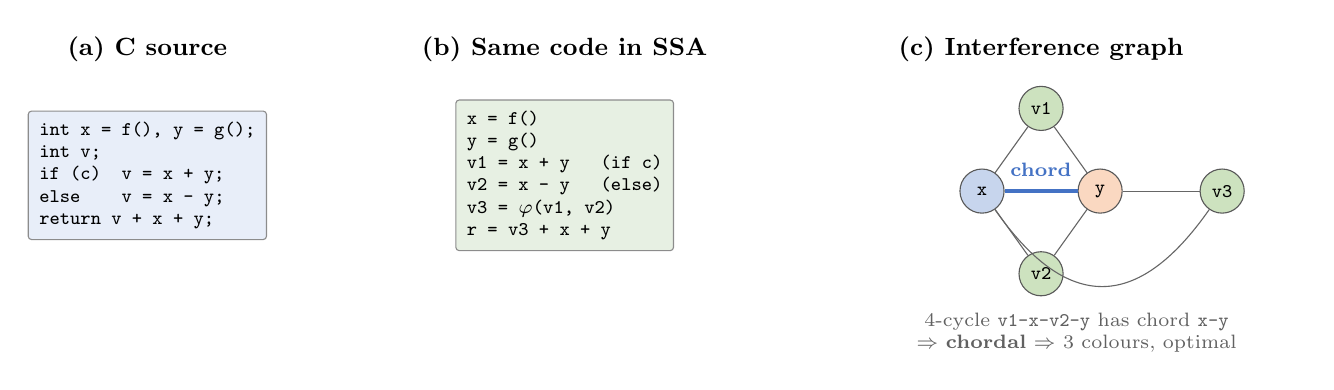
\begin{tikzpicture}[
  code/.style={draw=black!45,rounded corners=1.2pt,fill=lyrIn,align=left,
               inner sep=4pt,font=\scriptsize\ttfamily},
  ig/.style={draw=black!65,circle,inner sep=0pt,minimum size=0.56cm,font=\scriptsize},
  ed/.style={draw=black!60,thin},
  pcap/.style={font=\small\bfseries,align=center},
  ann/.style={font=\scriptsize,color=black!62,align=center}]

%---------------- (a) original C ----------------
\node[pcap] at (0,2.15) {(a) C source};
\node[code] (c1) at (0,0.55)
  {int x = f(), y = g();\\
   int v;\\
   if (c)\ \ v = x + y;\\
   else\ \ \ \ v = x - y;\\
   return v + x + y;};

%---------------- (b) SSA form ----------------
\begin{scope}[xshift=5.3cm]
  \node[pcap] at (0,2.15) {(b) Same code in SSA};
  \node[code,fill=lyrAna] (c2) at (0,0.55)
    {x\ = f()\\
     y\ = g()\\
     v1 = x + y\ \ \ (if c)\\
     v2 = x - y\ \ \ (else)\\
     v3 = $\varphi$(v1, v2)\\
     r\ = v3 + x + y};
\end{scope}

%---------------- (c) interference graph ----------------
\begin{scope}[xshift=10.6cm,yshift=0.35cm]
  \node[pcap] at (0.75,1.80) {(c) Interference graph};
  \node[ig,fill=regA!30] (vx)  at (0,0)        {\texttt{x}};
  \node[ig,fill=regB!30] (vy)  at (1.50,0)     {\texttt{y}};
  \node[ig,fill=regC!35] (v1)  at (0.75,1.05)  {\texttt{v1}};
  \node[ig,fill=regC!35] (v2)  at (0.75,-1.05) {\texttt{v2}};
  \node[ig,fill=regC!35] (v3)  at (3.05,0)     {\texttt{v3}};
  \draw[ed] (vx)--(v1); \draw[ed] (v1)--(vy);
  \draw[ed] (vx)--(v2); \draw[ed] (v2)--(vy);
  \draw[ed] (vy)--(v3);
  \draw[ed] (vx) to[out=-55,in=235,looseness=1.5] (v3);
  \draw[iiitkblue,line width=1.2pt] (vx)--(vy)
        node[midway,above=0.5mm,font=\scriptsize\bfseries,color=iiitkblue]{chord};
  \node[ann,text width=5.6cm] at (1.2,-1.80)
    {4-cycle \texttt{v1-x-v2-y} has chord \texttt{x-y} $\Rightarrow$
     \textbf{chordal} $\Rightarrow$ 3 colours, optimal};
\end{scope}
\end{tikzpicture}
\end{adjustbox}}

%----------------------------------------------------------------------
% 5. FIGURE 2 -- Slide 8: system pipeline, allocator is the swappable box
%----------------------------------------------------------------------
\newcommand{\FigPipeline}{%
\begin{adjustbox}{max width=\textwidth,max totalheight=6.0cm}
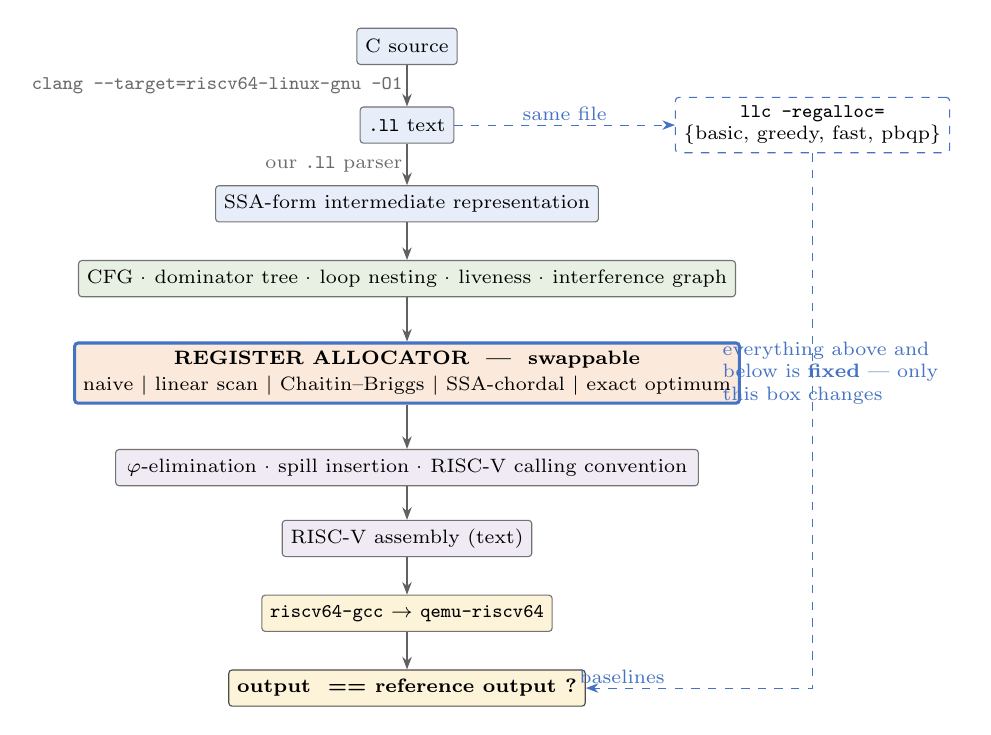
\begin{tikzpicture}[
  n/.style={draw=black!55,rounded corners=1.2pt,align=center,
            font=\scriptsize,inner sep=3pt,minimum height=0.46cm},
  wide/.style={n,minimum width=7.4cm},
  fl/.style={-{Stealth[length=1.6mm]},draw=black!62},
  lbl/.style={font=\scriptsize,color=black!58,inner sep=1.5pt}]

\node[n,fill=lyrIn]   (csrc) at (0, 0.00) {C source};
\node[n,fill=lyrIn]   (llt)  at (0,-1.00) {\texttt{.ll} text};
\node[n,fill=lyrIn]   (ir)   at (0,-2.00) {SSA-form intermediate representation};
\node[wide,fill=lyrAna] (ana) at (0,-2.95)
  {CFG \textperiodcentered\ dominator tree \textperiodcentered\ loop nesting
   \textperiodcentered\ liveness \textperiodcentered\ interference graph};
\node[wide,fill=lyrAlloc,draw=iiitkblue,line width=1.1pt] (alloc) at (0,-4.15)
  {\textbf{REGISTER ALLOCATOR \ --- \ swappable}\\[0.4mm]
   naive \textbar\ linear scan \textbar\ Chaitin--Briggs \textbar\
   SSA-chordal \textbar\ exact optimum};
\node[wide,fill=lyrBack] (back) at (0,-5.35)
  {$\varphi$-elimination \textperiodcentered\ spill insertion
   \textperiodcentered\ RISC-V calling convention};
\node[n,fill=lyrBack] (asm)  at (0,-6.25) {RISC-V assembly (text)};
\node[n,fill=lyrEval] (run)  at (0,-7.20)
  {\texttt{riscv64-gcc} $\rightarrow$ \texttt{qemu-riscv64}};
\node[n,fill=lyrEval,draw=black!70] (chk) at (0,-8.15)
  {\textbf{output \ ==\ reference output ?}};

\draw[fl] (csrc) -- node[lbl,left]{\texttt{clang --target=riscv64-linux-gnu -O1}} (llt);
\draw[fl] (llt)  -- node[lbl,left]{our \texttt{.ll} parser} (ir);
\draw[fl] (ir) -- (ana);
\draw[fl] (ana) -- (alloc);
\draw[fl] (alloc) -- (back);
\draw[fl] (back) -- (asm);
\draw[fl] (asm) -- (run);
\draw[fl] (run) -- (chk);

% fixed above and below: only the boxed allocator changes
\node[lbl,anchor=west,text width=3.0cm,align=left,color=iiitkblue]
     at (3.95,-4.15) {everything above and below is \textbf{fixed} --- only this box changes};

% external baselines off the same .ll
\node[n,fill=white,draw=regA,dashed,align=center] (llc) at (5.15,-1.00)
  {\texttt{llc -regalloc=}\\\{basic, greedy, fast, pbqp\}};
\draw[fl,draw=regA,dashed] (llt) -- node[lbl,above,color=regA]{same file} (llc);
\draw[fl,draw=regA,dashed] (llc) |- node[lbl,pos=0.92,above,color=regA]{baselines} (chk.east);
\end{tikzpicture}
\end{adjustbox}}

%======================================================================
\title{Design and Implementation of an SSA-Based RISC-V Compiler with
       Comparative Register Allocation}
\author{Shaun Alan Joseph \and Rishi Sharma \and Komal \and Aswin Parames}
\institute{Indian Institute of Information Technology Kottayam}
\date{9 September 2026}

\begin{document}

%======================= 1. TITLE =====================================
\begin{frame}
\vspace{0.9cm}
\begin{center}
{\large\textbf{Design and Implementation of an SSA-Based RISC-V Compiler\\[1mm]
 with Comparative Register Allocation}}\\[7mm]
{\footnotesize
\begin{tabular}{@{}c@{\hspace{7mm}}c@{\hspace{7mm}}c@{\hspace{7mm}}c@{}}
Shaun Alan Joseph & Rishi Sharma & Komal & Aswin Parames \\[0.4mm]
{\scriptsize\color{black!60}2023BCD0006} &
{\scriptsize\color{black!60}2023BCD0023} &
{\scriptsize\color{black!60}2023BCD0011} &
{\scriptsize\color{black!60}2023BCD0024} \\
\end{tabular}}\\[4mm]
{\footnotesize\textbf{Guided by:} Dr.\ Nandini J Warrier}\\[2mm]
{\footnotesize Dept.\ of Computer Science and Engineering}\\[1mm]
{\footnotesize Indian Institute of Information Technology, Kottayam}\\[5mm]
{\scriptsize\color{black!55} B.Tech Project \textperiodcentered\ Phase 1
 \textperiodcentered\ Review 1 \textperiodcentered\ 9 September 2026}
\end{center}
\end{frame}

%======================= 2. INTRODUCTION ==============================
\begin{frame}{Introduction: Register Allocation}
\textbf{The last big decision a compiler makes}
\begin{itemize}\small
  \item A program uses unlimited named values. A CPU has few \textbf{registers}
        --- 32 on RISC-V, 16 on x86-64
  \item Values that don't fit are \textbf{spilled} to memory. A spilled value
        costs a load and a store on \emph{every} access --- inside a loop,
        every iteration
  \item One of the highest-impact passes in a compiler backend
  \item \textbf{Chaitin (1981):} build an \textbf{interference graph} --- one
        node per value, an edge between values alive at the same time --- then
        colour it with \emph{k} colours, where \emph{k} = number of registers
\end{itemize}
\end{frame}

%======================= 3. SSA BACKGROUND ============================
\begin{frame}{Background: SSA Form}
\vspace{-1mm}
\begin{columns}[T]
\begin{column}{0.49\textwidth}
{\small\textbf{Static Single Assignment (SSA)}}
\begin{itemize}\scriptsize
  \item Every value assigned \textbf{exactly once}. Reassignment creates a new
        value: \texttt{x1}, \texttt{x2}, \texttt{x3}
  \item Where control flow merges, a \textbf{$\varphi$-function} picks whichever
        value arrived: \texttt{x3 = $\varphi$(x1, x2)}
  \item Used by LLVM, GCC, HotSpot, V8 --- the normal form of modern compilers
\end{itemize}
\end{column}
\begin{column}{0.49\textwidth}
{\small\textbf{Why SSA changes the problem}}
\begin{itemize}\scriptsize
  \item In general interference graphs can be \emph{any} shape, and colouring
        an arbitrary graph is NP-hard --- the textbook reason for heuristics
  \item Interference graphs of SSA programs are always \textbf{chordal}
  \item Chordal graphs colour \textbf{optimally, in linear time}
  \item Established by Hack \& Goos and by Pereira \& Palsberg, both 2005
\end{itemize}
\end{column}
\end{columns}
\vspace{2mm}
\centering\FigChordality
\end{frame}

%======================= 4a. LITERATURE (lines) =======================
\begin{frame}{Literature Survey}
\framesubtitle{Two lines of work}
\vspace{-1mm}
{\footnotesize\textbf{The classical line --- all heuristics, no optimality guarantee}}\par\vspace{1mm}
{\scriptsize
\begin{tabular}{@{}p{3.6cm}p{1.1cm}p{8.2cm}@{}}
\toprule
Work & Year & Contribution \\
\midrule
Chaitin et al.              & 1981 & Interference-graph formulation; showed the problem is NP-hard in general \\
Briggs, Cooper \& Torczon   & 1994 & \textbf{Optimistic colouring.} Ancestor of most production allocators \\
George \& Appel             & 1996 & Iterated coalescing --- removes redundant copy instructions \\
Poletto \& Sarkar           & 1999 & \textbf{Linear scan.} Drops graph colouring for speed; what JITs ship \\
\bottomrule
\end{tabular}}\par\vspace{2.5mm}
{\footnotesize\textbf{The SSA line --- and what it already established}}\par\vspace{1mm}
{\scriptsize
\begin{tabular}{@{}p{3.6cm}p{1.1cm}p{8.2cm}@{}}
\toprule
Work & Year & Contribution \\
\midrule
Tarjan \& Yannakakis          & 1984    & Linear-time chordality test and colouring order \\
\textbf{Hack \& Goos}         & 2005--06& SSA interference graphs are \textbf{chordal} $\Rightarrow$ optimal colouring in linear time \\
\textbf{Pereira \& Palsberg}  & 2005    & Built a chordal allocator, measured 23,681 Java methods. \textbf{$\sim$95\% of graphs are chordal} \\
Bouchez, Darte \& Rastello    & 2006    & The remaining hardness is in \textbf{spilling and coalescing}, not colouring \\
\bottomrule
\end{tabular}}
\end{frame}

%======================= 4b. LITERATURE (their numbers) ===============
\begin{frame}{Literature Survey}
\framesubtitle{Their measured results --- we reproduce these, we don't discover them}
\vspace{2mm}
\centering
{\footnotesize
\begin{tabular}{@{}p{5.4cm}p{7.4cm}@{}}
\toprule
Question & Published answer \emph{(Pereira \& Palsberg, Table 1)} \\
\midrule
Optimal vs.\ classical heuristic?          & \textbf{4.13 vs 4.17} registers/method --- under 1\% \\
Does $\varphi$-elimination destroy chordality? & \textbf{No --- it improves it.} 91\% $\rightarrow$ 95.5\% \\
Does the advantage survive few registers?  & Better at \emph{k}=6, roughly equal at \emph{k}=18 \\
\bottomrule
\end{tabular}}
\vspace{5mm}

\begin{minipage}{0.86\textwidth}\small
\textbf{We are not claiming to discover any of this.} These are the numbers we
expect to reproduce --- on a different processor, in our own compiler --- and
knowing them in advance is how we will tell whether our implementation is
correct.
\end{minipage}
\end{frame}

%======================= 5. MOTIVATION ================================
\begin{frame}{Motivation: Why Build Another One}
{\small\textbf{The algorithms are known. The comparison between them is not reliable.}}\par\vspace{2mm}
{\scriptsize Every published comparison used a different compiler, target and
benchmark set:}\par\vspace{1.5mm}
\centering
{\scriptsize
\begin{tabular}{@{}p{3.4cm}p{2.2cm}p{2.6cm}p{4.0cm}@{}}
\toprule
Work & Compiler & Target & Benchmarks \\
\midrule
Pereira \& Palsberg & JoeQ      & Java bytecode & Java standard library \\
Hack \& Goos        & libFirm   & x86           & SPEC \\
Poletto \& Sarkar   & their own & x86           & their own set \\
LLVM \texttt{greedy}& LLVM      & many          & LLVM's own suite \\
\bottomrule
\end{tabular}}\par\vspace{3mm}
\begin{minipage}{0.92\textwidth}\scriptsize
\textbf{So the numbers can't be placed side by side.} A difference between two
published results might be the algorithm --- or the compiler, the processor, or
the test programs.
\end{minipage}\par\vspace{2.5mm}
\begin{minipage}{0.92\textwidth}
{\small\textbf{What we build instead}}
\begin{itemize}\scriptsize
  \item \textbf{One} compiler, \textbf{one} IR, \textbf{one} benchmark set,
        \textbf{one} backend --- with the allocator as a swappable part
  \item Every difference in output is then caused by the algorithm and nothing else
  \item On \textbf{RISC-V}, where this comparison hasn't been published
\end{itemize}
\end{minipage}
\end{frame}

%======================= 6. PROBLEM STATEMENT =========================
\begin{frame}{Problem Statement}
\vspace{1mm}
\begin{minipage}{0.95\textwidth}
\small\textbf{Design and implement an SSA-based RISC-V compiler in which the
register allocator is a swappable component, implement five allocation
strategies, and compare them under identical conditions.}
\end{minipage}
\vspace{4mm}

{\small\textbf{Three things we measure}}
\begin{itemize}\small
  \item[\textbf{1}] \textbf{Allocation quality.} How many spills does each
        algorithm produce on the same program? Compared against LLVM's
        production allocators, and against a true optimum from an exact solver
        on small functions.
  \item[\textbf{2}] \textbf{Effect of register count.} RISC-V has two official
        integer register configurations --- \textbf{RV32I/RV64I with 32}, and
        \textbf{RV32E with 16}, used in embedded chips. We run every allocator
        on both. Real hardware, not an artificial setting.
  \item[\textbf{3}] \textbf{Cost of the algorithm.} How much work each allocator
        does, counted in operations rather than seconds, so the numbers
        reproduce on any machine.
\end{itemize}
\end{frame}

%======================= 7. SCOPE =====================================
\begin{frame}{Scope of Work}
\vspace{3mm}
\centering
{\footnotesize
\begin{tabular}{@{}p{2.1cm}p{10.6cm}@{}}
\toprule
Layer & Components \\
\midrule
Input      & Textual LLVM IR (\texttt{.ll}) parser, defined subset \\[0.8mm]
Analysis   & CFG \textperiodcentered\ dominator tree \textperiodcentered\ loop detection \textperiodcentered\ liveness \textperiodcentered\ interference graph \textperiodcentered\ chordality test \\[0.8mm]
Allocation & \textbf{Five allocators:} naive \textperiodcentered\ linear scan \textperiodcentered\ Chaitin--Briggs \textperiodcentered\ SSA/chordal \textperiodcentered\ exact optimum \textperiodcentered\ plus coalescing \\[0.8mm]
Backend    & $\varphi$-elimination \textperiodcentered\ spill insertion \textperiodcentered\ RISC-V calling convention \textperiodcentered\ assembly emission \\[0.8mm]
Validation & Static allocation verifier \textperiodcentered\ differential testing \textperiodcentered\ random program testing \\[0.8mm]
Evaluation & Metrics \textperiodcentered\ LLVM \texttt{llc} baselines \textperiodcentered\ 16- vs 32-register comparison \textperiodcentered\ plots \textperiodcentered\ graph visualiser \\
\bottomrule
\end{tabular}}
\vspace{5mm}

\begin{minipage}{0.93\textwidth}\footnotesize
\textbf{Beating LLVM's \texttt{greedy} is not a goal.} Landing within a
constant factor and explaining the gap is.
\end{minipage}
\end{frame}

%======================= 8. ARCHITECTURE ==============================
\begin{frame}{Proposed Architecture}
\vspace{0.5mm}
\centering\FigPipeline
\end{frame}

%======================= 9. FIVE ALLOCATORS ===========================
\begin{frame}{The Five Allocators}
{\scriptsize All five consume \textbf{the same interference graph} and
\textbf{the same register budget}. Any difference in output is caused by the
algorithm alone.}\par\vspace{2mm}
{\scriptsize
\begin{tabular}{@{}p{2.5cm}p{4.6cm}p{5.7cm}@{}}
\toprule
Allocator & What it does & Why it's in the study \\
\midrule
\textbf{Naive}            & Spill everything & Correctness floor. Gets the pipeline working before any real algorithm exists \\
\textbf{Linear scan} (1999)& One pass over live intervals, no graph & Speed baseline --- what JITs ship \\
\textbf{Chaitin--Briggs} (1981/94) & Build $\rightarrow$ simplify $\rightarrow$ optimistic spill $\rightarrow$ select & The classical heuristic. Main comparison point \\
\textbf{SSA / chordal} (2005) & Colour along the order from Maximum Cardinality Search & \textbf{Optimal colouring in linear time}, because SSA graphs are chordal \\
\textbf{Exact optimum}    & Integer linear program, off-the-shelf solver & Too slow for real use; small functions only, gives a \textbf{true reference point} \\
\emph{+ Coalescing} (1996)& Removes redundant copies & Add-on to the graph-based allocators \\
\bottomrule
\end{tabular}}\end{frame}

%======================= 10. EVALUATION ===============================
\begin{frame}{Evaluation and Correctness}
\vspace{-1mm}
\begin{columns}[T]
\begin{column}{0.56\textwidth}
{\scriptsize\textbf{Metrics} --- all counted, never wall-clock}\par\vspace{1mm}
{\scriptsize
\begin{tabular}{@{}p{3.3cm}p{3.6cm}@{}}
\toprule
Metric & What it tells us \\
\midrule
Static spill count & The headline quality number \\
Spills weighted by $10^{\text{loop depth}}$ & Standard proxy for real runtime cost \\
Distance from the exact optimum & How far each heuristic really is from best possible \\
Executed instruction count (QEMU) & End-to-end quality, deterministic \\
Allocator operations executed & Cost side of the quality/cost trade \\
\bottomrule
\end{tabular}}
\end{column}
\begin{column}{0.42\textwidth}
{\scriptsize\textbf{Register-count comparison} --- both are real RISC-V
configurations, not an artificial knob}\par\vspace{1mm}
{\scriptsize
\begin{tabular}{@{}p{2.1cm}p{3.1cm}@{}}
\toprule
Profile & Integer registers \\
\midrule
RV64I / RV32I & 32 \\
\textbf{RV32E} & \textbf{16} --- official embedded profile, high pressure \\
\bottomrule
\end{tabular}}\par\vspace{2mm}
{\scriptsize\textbf{Baselines:} \texttt{llc -regalloc=}\{basic, greedy, fast,
pbqp\} on \textbf{identical IR}}
\end{column}
\end{columns}
\vspace{2.5mm}
\begin{minipage}{0.97\textwidth}
{\scriptsize\textbf{Correctness --- an allocator that miscompiles silently
invalidates every number.} Three independent layers, starting week 1:}
\begin{enumerate}\scriptsize
  \item \textbf{Static verifier} --- checks the allocation without running
        anything: no two simultaneously-alive values share a register, spill
        slots don't overlap
  \item \textbf{Differential testing} --- every benchmark's output compared
        against the \texttt{clang} build of the same source
  \item \textbf{Random program generation} --- auto-generated C programs, output
        compared against GCC
\end{enumerate}
\end{minipage}
\end{frame}

%======================= 11. WORK PLAN ================================
\begin{frame}{Work Plan and Current Status}
\vspace{-1mm}
\begin{columns}[T]
\begin{column}{0.49\textwidth}
{\scriptsize\textbf{Phase 1 --- build the compiler (weeks 1--8)}}\par\vspace{1mm}
{\scriptsize
\begin{tabular}{@{}p{0.8cm}p{5.3cm}@{}}
\toprule
Weeks & Work \\
\midrule
1--2 & Toolchain \textperiodcentered\ end-to-end spike \textperiodcentered\ \texttt{.ll} parser \textperiodcentered\ IR structures \textperiodcentered\ CFG \\
3--4 & Dominator tree \textperiodcentered\ loop detection \textperiodcentered\ liveness \textperiodcentered\ interference graph \textperiodcentered\ naive allocator \\
5--6 & Linear scan \textperiodcentered\ Chaitin--Briggs \\
7--8 & $\varphi$-elimination \textperiodcentered\ RISC-V calling convention \textperiodcentered\ verifier \textperiodcentered\ differential testing \\
\bottomrule
\end{tabular}}
\end{column}
\begin{column}{0.49\textwidth}
{\scriptsize\textbf{Phase 2 --- the comparison (weeks 9--16)}}\par\vspace{1mm}
{\scriptsize
\begin{tabular}{@{}p{0.9cm}p{5.2cm}@{}}
\toprule
Weeks & Work \\
\midrule
9--10  & Benchmarks \textperiodcentered\ LLVM \texttt{llc} baselines \textperiodcentered\ SSA/chordal allocator \\
11--12 & Exact solver on small functions \textperiodcentered\ coalescing \\
13--14 & 16- vs 32-register comparison across all allocators \textperiodcentered\ slack \\
15--16 & Results \textperiodcentered\ visualiser \textperiodcentered\ report \\
\bottomrule
\end{tabular}}
\end{column}
\end{columns}
\vspace{3mm}
{\scriptsize\textbf{Current status}}
\begin{itemize}\scriptsize
  \item Title and scope finalised with the guide
  \item Core literature reviewed, including the specific numbers we expect to reproduce
  \item Architecture and module interfaces specified; work divided across four tracks
  \item \textbf{Toolchain validated end-to-end.} C $\rightarrow$ \texttt{clang}
        $\rightarrow$ RISC-V IR $\rightarrow$ \texttt{llc} $\rightarrow$ assembly
        $\rightarrow$ \texttt{riscv64-linux-gnu-gcc} $\rightarrow$
        \texttt{qemu-riscv64}, output identical to the host-compiled reference
  \item \textbf{All four LLVM baseline allocators confirmed on RISC-V --- and they
        already differentiate.} On a small loop kernel, \texttt{fast} emits
        \textbf{20} stack accesses where \texttt{basic}, \texttt{greedy} and
        \texttt{pbqp} emit \textbf{2}
\end{itemize}
\end{frame}

%======================= 12a. APPLICATIONS ============================
\begin{frame}{Applications}
\vspace{2mm}
\begin{itemize}\small
  \item \textbf{A controlled comparison that doesn't currently exist} --- five
        allocators, one compiler, one benchmark set, one target, so the numbers
        are actually comparable
  \item \textbf{RISC-V embedded toolchains} --- RV32E has only 16 registers.
        That's where allocator choice matters most, and it isn't well
        characterised
  \item \textbf{JIT compilers} --- linear scan is deployed because colouring is
        assumed expensive. On SSA, optimal colouring is linear-time; our
        operation counts are the data needed to revisit that
  \item \textbf{Reusable artefacts} --- a readable implementation of five
        allocators on a common IR (production allocators are effectively
        unreadable), a verification harness, and an interference-graph
        visualiser
\end{itemize}
\end{frame}

%======================= 12b. CONCLUSION ==============================
\begin{frame}{Conclusion}
\vspace{2mm}
\begin{itemize}\small
  \item Register allocation is classically graph colouring, NP-hard in general.
        \textbf{For SSA it isn't} --- optimal colouring is linear-time,
        established 2005
  \item The algorithms are known. \textbf{What's missing is a fair comparison}
        --- every published result comes from a different compiler, target and
        benchmark set
  \item We build an SSA-based RISC-V compiler with a \textbf{swappable}
        allocator, implement five strategies, and compare them on both RISC-V
        register profiles
  \item \textbf{Next phase:} complete the analysis layer and classical
        allocators, reach a correct end-to-end pipeline, begin the comparison
\end{itemize}
\vspace{4mm}
\centering{\small\color{black!55} Thank you --- questions welcome.}
\end{frame}

%======================= 13. REFERENCES ===============================
\begin{frame}{References}
\vspace{1mm}
{\scriptsize
\begin{enumerate}\setlength{\itemsep}{1.1mm}
\item G. J. Chaitin \emph{et al.}, ``Register allocation via coloring,''
      \emph{Computer Languages}, vol.\ 6, no.\ 1, pp.\ 47--57, 1981.
\item P. Briggs, K. D. Cooper, and L. Torczon, ``Improvements to graph coloring
      register allocation,'' \emph{ACM TOPLAS}, vol.\ 16, no.\ 3,
      pp.\ 428--455, 1994.
\item L. George and A. W. Appel, ``Iterated register coalescing,''
      \emph{ACM TOPLAS}, vol.\ 18, no.\ 3, pp.\ 300--324, 1996.
\item M. Poletto and V. Sarkar, ``Linear scan register allocation,''
      \emph{ACM TOPLAS}, vol.\ 21, no.\ 5, pp.\ 895--913, 1999.
\item S. Hack and G. Goos, ``Optimal register allocation for SSA-form programs
      in polynomial time,'' \emph{Inf.\ Process.\ Lett.}, vol.\ 98, no.\ 4,
      pp.\ 150--155, 2006.
\item F. M. Q. Pereira and J. Palsberg, ``Register allocation via coloring of
      chordal graphs,'' in \emph{Proc.\ APLAS}, 2005, pp.\ 315--329.
\item F. Bouchez, A. Darte, and F. Rastello, ``Register allocation: What does
      the NP-completeness proof of Chaitin et al.\ really prove?,'' in
      \emph{Proc.\ LCPC}, 2006, pp.\ 283--298.
\item R. E. Tarjan and M. Yannakakis, ``Simple linear-time algorithms to test
      chordality of graphs\dots,'' \emph{SIAM J.\ Comput.}, vol.\ 13, no.\ 3,
      pp.\ 566--579, 1984.
\item R. Casta\~{n}eda Lozano and C. Schulte, ``Survey on combinatorial register
      allocation and instruction scheduling,'' \emph{ACM Comput.\ Surv.},
      vol.\ 52, no.\ 3, 2019.
\end{enumerate}}
\end{frame}

\end{document}
" -> deck + speaker notes
%=======================================================================
\documentclass[aspectratio=169,11pt]{beamer}

\usepackage{fontspec}
% Carlito = metric clone of Calibri (the template's font).
% Resolved by family name (works locally via fontconfig) or by filename
% (works on Overleaf via the TeX Live tree). Warns loudly if neither works,
% rather than silently falling back to a font that isn't the template's.
\IfFontExistsTF{Carlito}{%
  \setsansfont{Carlito}%
}{%
  \IfFontExistsTF{Carlito-Regular.ttf}{%
    \setsansfont{Carlito}[Extension=.ttf,UprightFont=*-Regular,
      BoldFont=*-Bold,ItalicFont=*-Italic,BoldItalicFont=*-BoldItalic]%
  }{%
    \GenericWarning{}{** CARLITO NOT FOUND -- deck will not match the
      institute template. Install/enable the carlito font. **}%
  }%
}
\usepackage{booktabs}
\usepackage{adjustbox}
\usepackage{graphicx}
\usepackage{xcolor}
\usepackage{tikz}
\usetikzlibrary{arrows.meta,positioning,fit,backgrounds,calc,shapes.geometric}

%----------------------------------------------------------------------
% 1. COLOURS  (from the institute template's Office theme)
%----------------------------------------------------------------------
\definecolor{iiitkblue}{HTML}{4472C4}   % template accent1
\definecolor{iiitkdark}{HTML}{44546A}   % template dk2
\definecolor{regA}{HTML}{4472C4}
\definecolor{regB}{HTML}{ED7D31}
\definecolor{regC}{HTML}{70AD47}
\definecolor{lyrIn}{HTML}{E8EEF9}
\definecolor{lyrAna}{HTML}{E7F0E3}
\definecolor{lyrAlloc}{HTML}{FBE9DC}
\definecolor{lyrBack}{HTML}{EFEAF4}
\definecolor{lyrEval}{HTML}{FDF3D8}

%----------------------------------------------------------------------
% 2. THEME  (matches BTP Presentation Template-2-2.pptx)
%    white ground, black left-aligned titles, logo top-right,
%    centred institute footer, frame number bottom-right
%----------------------------------------------------------------------
\usetheme{default}
\setbeamercolor{normal text}{fg=black,bg=white}
\setbeamercolor{structure}{fg=iiitkblue}
\setbeamercolor{frametitle}{fg=black,bg=}
\setbeamercolor{itemize item}{fg=iiitkblue}
\setbeamercolor{itemize subitem}{fg=iiitkblue}
\setbeamertemplate{navigation symbols}{}
\setbeamertemplate{itemize item}{\raisebox{0.15ex}{\tiny$\bullet$}}
\setbeamertemplate{itemize subitem}{\raisebox{0.15ex}{\tiny$\circ$}}
\setbeamerfont{frametitle}{size=\large}
\setbeamerfont{framesubtitle}{size=\footnotesize}

% margins taken from the template master (1.10 cm at 16 cm slide width)
\setbeamersize{text margin left=1.1cm,text margin right=1.1cm}

% -- logo, placed at the template's exact coordinates, on every slide ---
\newcommand{\iiitklogo}{%
  \IfFileExists{iiitk-logo.jpeg}{\includegraphics[width=2.30cm]{iiitk-logo.jpeg}}{}}
\setbeamertemplate{background}{%
  \begin{tikzpicture}[overlay]
    \useasboundingbox (0,0) rectangle (\paperwidth,-\paperheight);
    \node[anchor=north east,inner sep=0pt]
      at ($(\paperwidth,0)+(-0.55cm,-0.10cm)$) {\iiitklogo};
  \end{tikzpicture}}

% -- frame title: black, left aligned, thin accent rule --------------
%    (delete the \rule line below for a pixel-plain template match)
\makeatletter
\setbeamertemplate{frametitle}{%
  \vspace{0.55cm}%
  \begin{minipage}{0.80\paperwidth}
    \raggedright\usebeamerfont{frametitle}\usebeamercolor[fg]{frametitle}%
    \insertframetitle\par
    \ifx\insertframesubtitle\@empty\else
      {\usebeamerfont{framesubtitle}\color{black!62}\insertframesubtitle\par}\fi
    \vspace{0.6mm}{\color{iiitkblue}\rule{\linewidth}{0.7pt}}
  \end{minipage}%
  \vspace{-0.15cm}}
\makeatother

\setbeamertemplate{footline}{%
  \hbox to \paperwidth{%
    \hspace*{1.1cm}%
    \hfill{\color{black!55}\fontsize{5.7}{7}\selectfont
           Indian Institute of Information Technology Kottayam}\hfill
    {\color{black!55}\fontsize{5.7}{7}\selectfont\insertframenumber}%
    \hspace*{1.1cm}}%
  \vspace{1.6mm}}

%----------------------------------------------------------------------
% 4. FIGURE 1 -- Slide 3: C code -> SSA with phi -> interference graph
%----------------------------------------------------------------------
\newcommand{\FigChordality}{%
\begin{adjustbox}{max width=\textwidth,max totalheight=3.1cm}
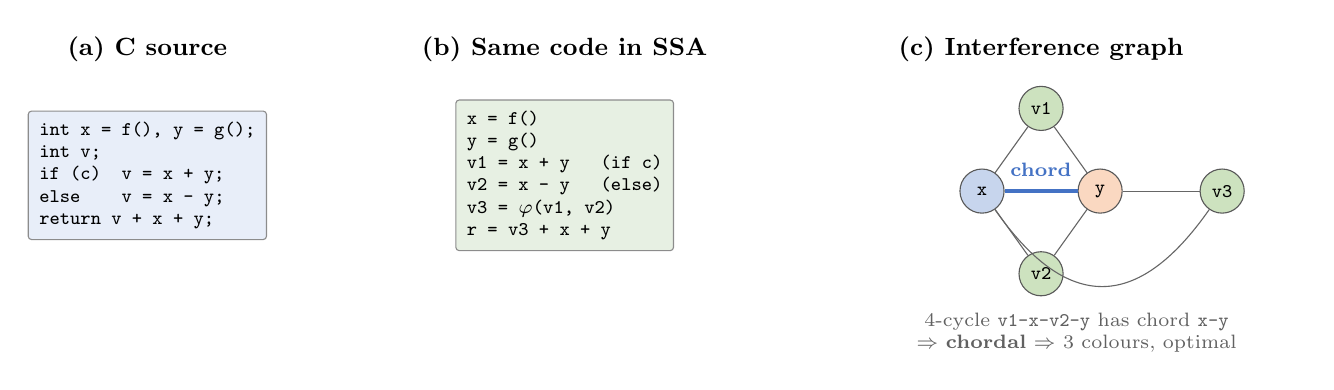
\begin{tikzpicture}[
  code/.style={draw=black!45,rounded corners=1.2pt,fill=lyrIn,align=left,
               inner sep=4pt,font=\scriptsize\ttfamily},
  ig/.style={draw=black!65,circle,inner sep=0pt,minimum size=0.56cm,font=\scriptsize},
  ed/.style={draw=black!60,thin},
  pcap/.style={font=\small\bfseries,align=center},
  ann/.style={font=\scriptsize,color=black!62,align=center}]

%---------------- (a) original C ----------------
\node[pcap] at (0,2.15) {(a) C source};
\node[code] (c1) at (0,0.55)
  {int x = f(), y = g();\\
   int v;\\
   if (c)\ \ v = x + y;\\
   else\ \ \ \ v = x - y;\\
   return v + x + y;};

%---------------- (b) SSA form ----------------
\begin{scope}[xshift=5.3cm]
  \node[pcap] at (0,2.15) {(b) Same code in SSA};
  \node[code,fill=lyrAna] (c2) at (0,0.55)
    {x\ = f()\\
     y\ = g()\\
     v1 = x + y\ \ \ (if c)\\
     v2 = x - y\ \ \ (else)\\
     v3 = $\varphi$(v1, v2)\\
     r\ = v3 + x + y};
\end{scope}

%---------------- (c) interference graph ----------------
\begin{scope}[xshift=10.6cm,yshift=0.35cm]
  \node[pcap] at (0.75,1.80) {(c) Interference graph};
  \node[ig,fill=regA!30] (vx)  at (0,0)        {\texttt{x}};
  \node[ig,fill=regB!30] (vy)  at (1.50,0)     {\texttt{y}};
  \node[ig,fill=regC!35] (v1)  at (0.75,1.05)  {\texttt{v1}};
  \node[ig,fill=regC!35] (v2)  at (0.75,-1.05) {\texttt{v2}};
  \node[ig,fill=regC!35] (v3)  at (3.05,0)     {\texttt{v3}};
  \draw[ed] (vx)--(v1); \draw[ed] (v1)--(vy);
  \draw[ed] (vx)--(v2); \draw[ed] (v2)--(vy);
  \draw[ed] (vy)--(v3);
  \draw[ed] (vx) to[out=-55,in=235,looseness=1.5] (v3);
  \draw[iiitkblue,line width=1.2pt] (vx)--(vy)
        node[midway,above=0.5mm,font=\scriptsize\bfseries,color=iiitkblue]{chord};
  \node[ann,text width=5.6cm] at (1.2,-1.80)
    {4-cycle \texttt{v1-x-v2-y} has chord \texttt{x-y} $\Rightarrow$
     \textbf{chordal} $\Rightarrow$ 3 colours, optimal};
\end{scope}
\end{tikzpicture}
\end{adjustbox}}

%----------------------------------------------------------------------
% 5. FIGURE 2 -- Slide 8: system pipeline, allocator is the swappable box
%----------------------------------------------------------------------
\newcommand{\FigPipeline}{%
\begin{adjustbox}{max width=\textwidth,max totalheight=6.0cm}
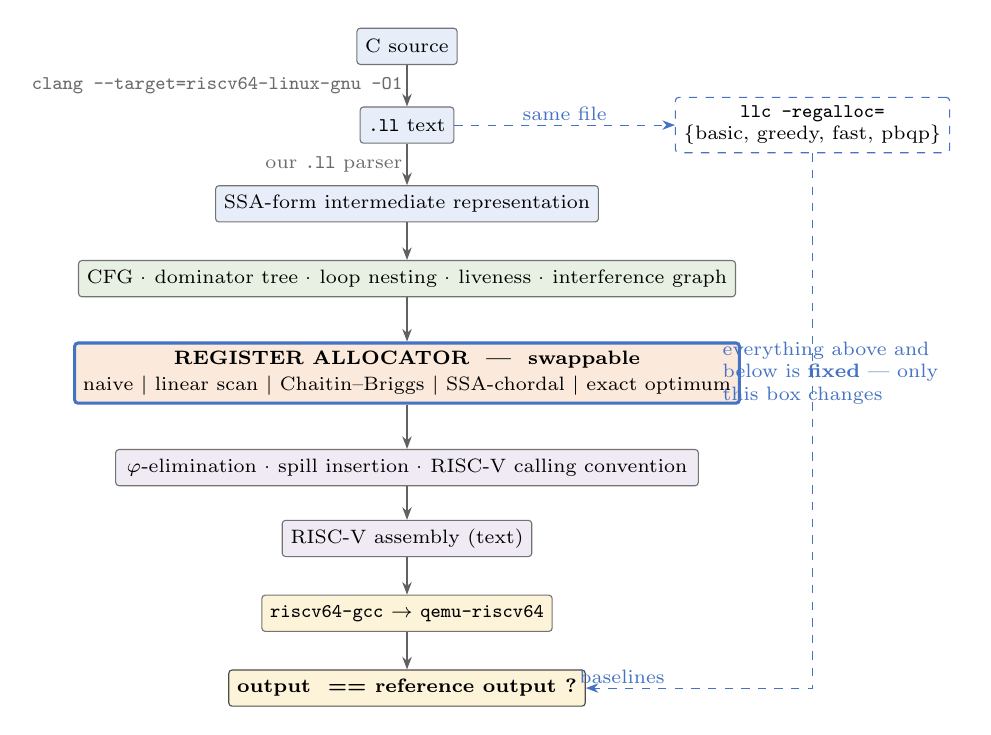
\begin{tikzpicture}[
  n/.style={draw=black!55,rounded corners=1.2pt,align=center,
            font=\scriptsize,inner sep=3pt,minimum height=0.46cm},
  wide/.style={n,minimum width=7.4cm},
  fl/.style={-{Stealth[length=1.6mm]},draw=black!62},
  lbl/.style={font=\scriptsize,color=black!58,inner sep=1.5pt}]

\node[n,fill=lyrIn]   (csrc) at (0, 0.00) {C source};
\node[n,fill=lyrIn]   (llt)  at (0,-1.00) {\texttt{.ll} text};
\node[n,fill=lyrIn]   (ir)   at (0,-2.00) {SSA-form intermediate representation};
\node[wide,fill=lyrAna] (ana) at (0,-2.95)
  {CFG \textperiodcentered\ dominator tree \textperiodcentered\ loop nesting
   \textperiodcentered\ liveness \textperiodcentered\ interference graph};
\node[wide,fill=lyrAlloc,draw=iiitkblue,line width=1.1pt] (alloc) at (0,-4.15)
  {\textbf{REGISTER ALLOCATOR \ --- \ swappable}\\[0.4mm]
   naive \textbar\ linear scan \textbar\ Chaitin--Briggs \textbar\
   SSA-chordal \textbar\ exact optimum};
\node[wide,fill=lyrBack] (back) at (0,-5.35)
  {$\varphi$-elimination \textperiodcentered\ spill insertion
   \textperiodcentered\ RISC-V calling convention};
\node[n,fill=lyrBack] (asm)  at (0,-6.25) {RISC-V assembly (text)};
\node[n,fill=lyrEval] (run)  at (0,-7.20)
  {\texttt{riscv64-gcc} $\rightarrow$ \texttt{qemu-riscv64}};
\node[n,fill=lyrEval,draw=black!70] (chk) at (0,-8.15)
  {\textbf{output \ ==\ reference output ?}};

\draw[fl] (csrc) -- node[lbl,left]{\texttt{clang --target=riscv64-linux-gnu -O1}} (llt);
\draw[fl] (llt)  -- node[lbl,left]{our \texttt{.ll} parser} (ir);
\draw[fl] (ir) -- (ana);
\draw[fl] (ana) -- (alloc);
\draw[fl] (alloc) -- (back);
\draw[fl] (back) -- (asm);
\draw[fl] (asm) -- (run);
\draw[fl] (run) -- (chk);

% fixed above and below: only the boxed allocator changes
\node[lbl,anchor=west,text width=3.0cm,align=left,color=iiitkblue]
     at (3.95,-4.15) {everything above and below is \textbf{fixed} --- only this box changes};

% external baselines off the same .ll
\node[n,fill=white,draw=regA,dashed,align=center] (llc) at (5.15,-1.00)
  {\texttt{llc -regalloc=}\\\{basic, greedy, fast, pbqp\}};
\draw[fl,draw=regA,dashed] (llt) -- node[lbl,above,color=regA]{same file} (llc);
\draw[fl,draw=regA,dashed] (llc) |- node[lbl,pos=0.92,above,color=regA]{baselines} (chk.east);
\end{tikzpicture}
\end{adjustbox}}

%======================================================================
\title{Design and Implementation of an SSA-Based RISC-V Compiler with
       Comparative Register Allocation}
\author{Shaun Alan Joseph \and Rishi Sharma \and Komal \and Aswin Parames}
\institute{Indian Institute of Information Technology Kottayam}
\date{9 September 2026}

\begin{document}

%======================= 1. TITLE =====================================
\begin{frame}
\vspace{0.9cm}
\begin{center}
{\large\textbf{Design and Implementation of an SSA-Based RISC-V Compiler\\[1mm]
 with Comparative Register Allocation}}\\[7mm]
{\footnotesize
\begin{tabular}{@{}c@{\hspace{7mm}}c@{\hspace{7mm}}c@{\hspace{7mm}}c@{}}
Shaun Alan Joseph & Rishi Sharma & Komal & Aswin Parames \\[0.4mm]
{\scriptsize\color{black!60}2023BCD0006} &
{\scriptsize\color{black!60}2023BCD0023} &
{\scriptsize\color{black!60}2023BCD0011} &
{\scriptsize\color{black!60}2023BCD0024} \\
\end{tabular}}\\[4mm]
{\footnotesize\textbf{Guided by:} Dr.\ Nandini J Warrier}\\[2mm]
{\footnotesize Dept.\ of Computer Science and Engineering}\\[1mm]
{\footnotesize Indian Institute of Information Technology, Kottayam}\\[5mm]
{\scriptsize\color{black!55} B.Tech Project \textperiodcentered\ Phase 1
 \textperiodcentered\ Review 1 \textperiodcentered\ 9 September 2026}
\end{center}
\end{frame}

%======================= 2. INTRODUCTION ==============================
\begin{frame}{Introduction: Register Allocation}
\textbf{The last big decision a compiler makes}
\begin{itemize}\small
  \item A program uses unlimited named values. A CPU has few \textbf{registers}
        --- 32 on RISC-V, 16 on x86-64
  \item Values that don't fit are \textbf{spilled} to memory. A spilled value
        costs a load and a store on \emph{every} access --- inside a loop,
        every iteration
  \item One of the highest-impact passes in a compiler backend
  \item \textbf{Chaitin (1981):} build an \textbf{interference graph} --- one
        node per value, an edge between values alive at the same time --- then
        colour it with \emph{k} colours, where \emph{k} = number of registers
\end{itemize}
\end{frame}

%======================= 3. SSA BACKGROUND ============================
\begin{frame}{Background: SSA Form}
\vspace{-1mm}
\begin{columns}[T]
\begin{column}{0.49\textwidth}
{\small\textbf{Static Single Assignment (SSA)}}
\begin{itemize}\scriptsize
  \item Every value assigned \textbf{exactly once}. Reassignment creates a new
        value: \texttt{x1}, \texttt{x2}, \texttt{x3}
  \item Where control flow merges, a \textbf{$\varphi$-function} picks whichever
        value arrived: \texttt{x3 = $\varphi$(x1, x2)}
  \item Used by LLVM, GCC, HotSpot, V8 --- the normal form of modern compilers
\end{itemize}
\end{column}
\begin{column}{0.49\textwidth}
{\small\textbf{Why SSA changes the problem}}
\begin{itemize}\scriptsize
  \item In general interference graphs can be \emph{any} shape, and colouring
        an arbitrary graph is NP-hard --- the textbook reason for heuristics
  \item Interference graphs of SSA programs are always \textbf{chordal}
  \item Chordal graphs colour \textbf{optimally, in linear time}
  \item Established by Hack \& Goos and by Pereira \& Palsberg, both 2005
\end{itemize}
\end{column}
\end{columns}
\vspace{2mm}
\centering\FigChordality
\end{frame}

%======================= 4a. LITERATURE (lines) =======================
\begin{frame}{Literature Survey}
\framesubtitle{Two lines of work}
\vspace{-1mm}
{\footnotesize\textbf{The classical line --- all heuristics, no optimality guarantee}}\par\vspace{1mm}
{\scriptsize
\begin{tabular}{@{}p{3.6cm}p{1.1cm}p{8.2cm}@{}}
\toprule
Work & Year & Contribution \\
\midrule
Chaitin et al.              & 1981 & Interference-graph formulation; showed the problem is NP-hard in general \\
Briggs, Cooper \& Torczon   & 1994 & \textbf{Optimistic colouring.} Ancestor of most production allocators \\
George \& Appel             & 1996 & Iterated coalescing --- removes redundant copy instructions \\
Poletto \& Sarkar           & 1999 & \textbf{Linear scan.} Drops graph colouring for speed; what JITs ship \\
\bottomrule
\end{tabular}}\par\vspace{2.5mm}
{\footnotesize\textbf{The SSA line --- and what it already established}}\par\vspace{1mm}
{\scriptsize
\begin{tabular}{@{}p{3.6cm}p{1.1cm}p{8.2cm}@{}}
\toprule
Work & Year & Contribution \\
\midrule
Tarjan \& Yannakakis          & 1984    & Linear-time chordality test and colouring order \\
\textbf{Hack \& Goos}         & 2005--06& SSA interference graphs are \textbf{chordal} $\Rightarrow$ optimal colouring in linear time \\
\textbf{Pereira \& Palsberg}  & 2005    & Built a chordal allocator, measured 23,681 Java methods. \textbf{$\sim$95\% of graphs are chordal} \\
Bouchez, Darte \& Rastello    & 2006    & The remaining hardness is in \textbf{spilling and coalescing}, not colouring \\
\bottomrule
\end{tabular}}
\end{frame}

%======================= 4b. LITERATURE (their numbers) ===============
\begin{frame}{Literature Survey}
\framesubtitle{Their measured results --- we reproduce these, we don't discover them}
\vspace{2mm}
\centering
{\footnotesize
\begin{tabular}{@{}p{5.4cm}p{7.4cm}@{}}
\toprule
Question & Published answer \emph{(Pereira \& Palsberg, Table 1)} \\
\midrule
Optimal vs.\ classical heuristic?          & \textbf{4.13 vs 4.17} registers/method --- under 1\% \\
Does $\varphi$-elimination destroy chordality? & \textbf{No --- it improves it.} 91\% $\rightarrow$ 95.5\% \\
Does the advantage survive few registers?  & Better at \emph{k}=6, roughly equal at \emph{k}=18 \\
\bottomrule
\end{tabular}}
\vspace{5mm}

\begin{minipage}{0.86\textwidth}\small
\textbf{We are not claiming to discover any of this.} These are the numbers we
expect to reproduce --- on a different processor, in our own compiler --- and
knowing them in advance is how we will tell whether our implementation is
correct.
\end{minipage}
\end{frame}

%======================= 5. MOTIVATION ================================
\begin{frame}{Motivation: Why Build Another One}
{\small\textbf{The algorithms are known. The comparison between them is not reliable.}}\par\vspace{2mm}
{\scriptsize Every published comparison used a different compiler, target and
benchmark set:}\par\vspace{1.5mm}
\centering
{\scriptsize
\begin{tabular}{@{}p{3.4cm}p{2.2cm}p{2.6cm}p{4.0cm}@{}}
\toprule
Work & Compiler & Target & Benchmarks \\
\midrule
Pereira \& Palsberg & JoeQ      & Java bytecode & Java standard library \\
Hack \& Goos        & libFirm   & x86           & SPEC \\
Poletto \& Sarkar   & their own & x86           & their own set \\
LLVM \texttt{greedy}& LLVM      & many          & LLVM's own suite \\
\bottomrule
\end{tabular}}\par\vspace{3mm}
\begin{minipage}{0.92\textwidth}\scriptsize
\textbf{So the numbers can't be placed side by side.} A difference between two
published results might be the algorithm --- or the compiler, the processor, or
the test programs.
\end{minipage}\par\vspace{2.5mm}
\begin{minipage}{0.92\textwidth}
{\small\textbf{What we build instead}}
\begin{itemize}\scriptsize
  \item \textbf{One} compiler, \textbf{one} IR, \textbf{one} benchmark set,
        \textbf{one} backend --- with the allocator as a swappable part
  \item Every difference in output is then caused by the algorithm and nothing else
  \item On \textbf{RISC-V}, where this comparison hasn't been published
\end{itemize}
\end{minipage}
\end{frame}

%======================= 6. PROBLEM STATEMENT =========================
\begin{frame}{Problem Statement}
\vspace{1mm}
\begin{minipage}{0.95\textwidth}
\small\textbf{Design and implement an SSA-based RISC-V compiler in which the
register allocator is a swappable component, implement five allocation
strategies, and compare them under identical conditions.}
\end{minipage}
\vspace{4mm}

{\small\textbf{Three things we measure}}
\begin{itemize}\small
  \item[\textbf{1}] \textbf{Allocation quality.} How many spills does each
        algorithm produce on the same program? Compared against LLVM's
        production allocators, and against a true optimum from an exact solver
        on small functions.
  \item[\textbf{2}] \textbf{Effect of register count.} RISC-V has two official
        integer register configurations --- \textbf{RV32I/RV64I with 32}, and
        \textbf{RV32E with 16}, used in embedded chips. We run every allocator
        on both. Real hardware, not an artificial setting.
  \item[\textbf{3}] \textbf{Cost of the algorithm.} How much work each allocator
        does, counted in operations rather than seconds, so the numbers
        reproduce on any machine.
\end{itemize}
\end{frame}

%======================= 7. SCOPE =====================================
\begin{frame}{Scope of Work}
\vspace{3mm}
\centering
{\footnotesize
\begin{tabular}{@{}p{2.1cm}p{10.6cm}@{}}
\toprule
Layer & Components \\
\midrule
Input      & Textual LLVM IR (\texttt{.ll}) parser, defined subset \\[0.8mm]
Analysis   & CFG \textperiodcentered\ dominator tree \textperiodcentered\ loop detection \textperiodcentered\ liveness \textperiodcentered\ interference graph \textperiodcentered\ chordality test \\[0.8mm]
Allocation & \textbf{Five allocators:} naive \textperiodcentered\ linear scan \textperiodcentered\ Chaitin--Briggs \textperiodcentered\ SSA/chordal \textperiodcentered\ exact optimum \textperiodcentered\ plus coalescing \\[0.8mm]
Backend    & $\varphi$-elimination \textperiodcentered\ spill insertion \textperiodcentered\ RISC-V calling convention \textperiodcentered\ assembly emission \\[0.8mm]
Validation & Static allocation verifier \textperiodcentered\ differential testing \textperiodcentered\ random program testing \\[0.8mm]
Evaluation & Metrics \textperiodcentered\ LLVM \texttt{llc} baselines \textperiodcentered\ 16- vs 32-register comparison \textperiodcentered\ plots \textperiodcentered\ graph visualiser \\
\bottomrule
\end{tabular}}
\vspace{5mm}

\begin{minipage}{0.93\textwidth}\footnotesize
\textbf{Beating LLVM's \texttt{greedy} is not a goal.} Landing within a
constant factor and explaining the gap is.
\end{minipage}
\end{frame}

%======================= 8. ARCHITECTURE ==============================
\begin{frame}{Proposed Architecture}
\vspace{0.5mm}
\centering\FigPipeline
\end{frame}

%======================= 9. FIVE ALLOCATORS ===========================
\begin{frame}{The Five Allocators}
{\scriptsize All five consume \textbf{the same interference graph} and
\textbf{the same register budget}. Any difference in output is caused by the
algorithm alone.}\par\vspace{2mm}
{\scriptsize
\begin{tabular}{@{}p{2.5cm}p{4.6cm}p{5.7cm}@{}}
\toprule
Allocator & What it does & Why it's in the study \\
\midrule
\textbf{Naive}            & Spill everything & Correctness floor. Gets the pipeline working before any real algorithm exists \\
\textbf{Linear scan} (1999)& One pass over live intervals, no graph & Speed baseline --- what JITs ship \\
\textbf{Chaitin--Briggs} (1981/94) & Build $\rightarrow$ simplify $\rightarrow$ optimistic spill $\rightarrow$ select & The classical heuristic. Main comparison point \\
\textbf{SSA / chordal} (2005) & Colour along the order from Maximum Cardinality Search & \textbf{Optimal colouring in linear time}, because SSA graphs are chordal \\
\textbf{Exact optimum}    & Integer linear program, off-the-shelf solver & Too slow for real use; small functions only, gives a \textbf{true reference point} \\
\emph{+ Coalescing} (1996)& Removes redundant copies & Add-on to the graph-based allocators \\
\bottomrule
\end{tabular}}\end{frame}

%======================= 10. EVALUATION ===============================
\begin{frame}{Evaluation and Correctness}
\vspace{-1mm}
\begin{columns}[T]
\begin{column}{0.56\textwidth}
{\scriptsize\textbf{Metrics} --- all counted, never wall-clock}\par\vspace{1mm}
{\scriptsize
\begin{tabular}{@{}p{3.3cm}p{3.6cm}@{}}
\toprule
Metric & What it tells us \\
\midrule
Static spill count & The headline quality number \\
Spills weighted by $10^{\text{loop depth}}$ & Standard proxy for real runtime cost \\
Distance from the exact optimum & How far each heuristic really is from best possible \\
Executed instruction count (QEMU) & End-to-end quality, deterministic \\
Allocator operations executed & Cost side of the quality/cost trade \\
\bottomrule
\end{tabular}}
\end{column}
\begin{column}{0.42\textwidth}
{\scriptsize\textbf{Register-count comparison} --- both are real RISC-V
configurations, not an artificial knob}\par\vspace{1mm}
{\scriptsize
\begin{tabular}{@{}p{2.1cm}p{3.1cm}@{}}
\toprule
Profile & Integer registers \\
\midrule
RV64I / RV32I & 32 \\
\textbf{RV32E} & \textbf{16} --- official embedded profile, high pressure \\
\bottomrule
\end{tabular}}\par\vspace{2mm}
{\scriptsize\textbf{Baselines:} \texttt{llc -regalloc=}\{basic, greedy, fast,
pbqp\} on \textbf{identical IR}}
\end{column}
\end{columns}
\vspace{2.5mm}
\begin{minipage}{0.97\textwidth}
{\scriptsize\textbf{Correctness --- an allocator that miscompiles silently
invalidates every number.} Three independent layers, starting week 1:}
\begin{enumerate}\scriptsize
  \item \textbf{Static verifier} --- checks the allocation without running
        anything: no two simultaneously-alive values share a register, spill
        slots don't overlap
  \item \textbf{Differential testing} --- every benchmark's output compared
        against the \texttt{clang} build of the same source
  \item \textbf{Random program generation} --- auto-generated C programs, output
        compared against GCC
\end{enumerate}
\end{minipage}
\end{frame}

%======================= 11. WORK PLAN ================================
\begin{frame}{Work Plan and Current Status}
\vspace{-1mm}
\begin{columns}[T]
\begin{column}{0.49\textwidth}
{\scriptsize\textbf{Phase 1 --- build the compiler (weeks 1--8)}}\par\vspace{1mm}
{\scriptsize
\begin{tabular}{@{}p{0.8cm}p{5.3cm}@{}}
\toprule
Weeks & Work \\
\midrule
1--2 & Toolchain \textperiodcentered\ end-to-end spike \textperiodcentered\ \texttt{.ll} parser \textperiodcentered\ IR structures \textperiodcentered\ CFG \\
3--4 & Dominator tree \textperiodcentered\ loop detection \textperiodcentered\ liveness \textperiodcentered\ interference graph \textperiodcentered\ naive allocator \\
5--6 & Linear scan \textperiodcentered\ Chaitin--Briggs \\
7--8 & $\varphi$-elimination \textperiodcentered\ RISC-V calling convention \textperiodcentered\ verifier \textperiodcentered\ differential testing \\
\bottomrule
\end{tabular}}
\end{column}
\begin{column}{0.49\textwidth}
{\scriptsize\textbf{Phase 2 --- the comparison (weeks 9--16)}}\par\vspace{1mm}
{\scriptsize
\begin{tabular}{@{}p{0.9cm}p{5.2cm}@{}}
\toprule
Weeks & Work \\
\midrule
9--10  & Benchmarks \textperiodcentered\ LLVM \texttt{llc} baselines \textperiodcentered\ SSA/chordal allocator \\
11--12 & Exact solver on small functions \textperiodcentered\ coalescing \\
13--14 & 16- vs 32-register comparison across all allocators \textperiodcentered\ slack \\
15--16 & Results \textperiodcentered\ visualiser \textperiodcentered\ report \\
\bottomrule
\end{tabular}}
\end{column}
\end{columns}
\vspace{3mm}
{\scriptsize\textbf{Current status}}
\begin{itemize}\scriptsize
  \item Title and scope finalised with the guide
  \item Core literature reviewed, including the specific numbers we expect to reproduce
  \item Architecture and module interfaces specified; work divided across four tracks
  \item \textbf{Toolchain validated end-to-end.} C $\rightarrow$ \texttt{clang}
        $\rightarrow$ RISC-V IR $\rightarrow$ \texttt{llc} $\rightarrow$ assembly
        $\rightarrow$ \texttt{riscv64-linux-gnu-gcc} $\rightarrow$
        \texttt{qemu-riscv64}, output identical to the host-compiled reference
  \item \textbf{All four LLVM baseline allocators confirmed on RISC-V --- and they
        already differentiate.} On a small loop kernel, \texttt{fast} emits
        \textbf{20} stack accesses where \texttt{basic}, \texttt{greedy} and
        \texttt{pbqp} emit \textbf{2}
\end{itemize}
\end{frame}

%======================= 12a. APPLICATIONS ============================
\begin{frame}{Applications}
\vspace{2mm}
\begin{itemize}\small
  \item \textbf{A controlled comparison that doesn't currently exist} --- five
        allocators, one compiler, one benchmark set, one target, so the numbers
        are actually comparable
  \item \textbf{RISC-V embedded toolchains} --- RV32E has only 16 registers.
        That's where allocator choice matters most, and it isn't well
        characterised
  \item \textbf{JIT compilers} --- linear scan is deployed because colouring is
        assumed expensive. On SSA, optimal colouring is linear-time; our
        operation counts are the data needed to revisit that
  \item \textbf{Reusable artefacts} --- a readable implementation of five
        allocators on a common IR (production allocators are effectively
        unreadable), a verification harness, and an interference-graph
        visualiser
\end{itemize}
\end{frame}

%======================= 12b. CONCLUSION ==============================
\begin{frame}{Conclusion}
\vspace{2mm}
\begin{itemize}\small
  \item Register allocation is classically graph colouring, NP-hard in general.
        \textbf{For SSA it isn't} --- optimal colouring is linear-time,
        established 2005
  \item The algorithms are known. \textbf{What's missing is a fair comparison}
        --- every published result comes from a different compiler, target and
        benchmark set
  \item We build an SSA-based RISC-V compiler with a \textbf{swappable}
        allocator, implement five strategies, and compare them on both RISC-V
        register profiles
  \item \textbf{Next phase:} complete the analysis layer and classical
        allocators, reach a correct end-to-end pipeline, begin the comparison
\end{itemize}
\vspace{4mm}
\centering{\small\color{black!55} Thank you --- questions welcome.}
\end{frame}

%======================= 13. REFERENCES ===============================
\begin{frame}{References}
\vspace{1mm}
{\scriptsize
\begin{enumerate}\setlength{\itemsep}{1.1mm}
\item G. J. Chaitin \emph{et al.}, ``Register allocation via coloring,''
      \emph{Computer Languages}, vol.\ 6, no.\ 1, pp.\ 47--57, 1981.
\item P. Briggs, K. D. Cooper, and L. Torczon, ``Improvements to graph coloring
      register allocation,'' \emph{ACM TOPLAS}, vol.\ 16, no.\ 3,
      pp.\ 428--455, 1994.
\item L. George and A. W. Appel, ``Iterated register coalescing,''
      \emph{ACM TOPLAS}, vol.\ 18, no.\ 3, pp.\ 300--324, 1996.
\item M. Poletto and V. Sarkar, ``Linear scan register allocation,''
      \emph{ACM TOPLAS}, vol.\ 21, no.\ 5, pp.\ 895--913, 1999.
\item S. Hack and G. Goos, ``Optimal register allocation for SSA-form programs
      in polynomial time,'' \emph{Inf.\ Process.\ Lett.}, vol.\ 98, no.\ 4,
      pp.\ 150--155, 2006.
\item F. M. Q. Pereira and J. Palsberg, ``Register allocation via coloring of
      chordal graphs,'' in \emph{Proc.\ APLAS}, 2005, pp.\ 315--329.
\item F. Bouchez, A. Darte, and F. Rastello, ``Register allocation: What does
      the NP-completeness proof of Chaitin et al.\ really prove?,'' in
      \emph{Proc.\ LCPC}, 2006, pp.\ 283--298.
\item R. E. Tarjan and M. Yannakakis, ``Simple linear-time algorithms to test
      chordality of graphs\dots,'' \emph{SIAM J.\ Comput.}, vol.\ 13, no.\ 3,
      pp.\ 566--579, 1984.
\item R. Casta\~{n}eda Lozano and C. Schulte, ``Survey on combinatorial register
      allocation and instruction scheduling,'' \emph{ACM Comput.\ Surv.},
      vol.\ 52, no.\ 3, 2019.
\end{enumerate}}
\end{frame}

\end{document}
" -> deck + speaker notes
%=======================================================================
\documentclass[aspectratio=169,11pt]{beamer}

\usepackage{fontspec}
% Carlito = metric clone of Calibri (the template's font).
% Resolved by family name (works locally via fontconfig) or by filename
% (works on Overleaf via the TeX Live tree). Warns loudly if neither works,
% rather than silently falling back to a font that isn't the template's.
\IfFontExistsTF{Carlito}{%
  \setsansfont{Carlito}%
}{%
  \IfFontExistsTF{Carlito-Regular.ttf}{%
    \setsansfont{Carlito}[Extension=.ttf,UprightFont=*-Regular,
      BoldFont=*-Bold,ItalicFont=*-Italic,BoldItalicFont=*-BoldItalic]%
  }{%
    \GenericWarning{}{** CARLITO NOT FOUND -- deck will not match the
      institute template. Install/enable the carlito font. **}%
  }%
}
\usepackage{booktabs}
\usepackage{adjustbox}
\usepackage{graphicx}
\usepackage{xcolor}
\usepackage{tikz}
\usetikzlibrary{arrows.meta,positioning,fit,backgrounds,calc,shapes.geometric}

%----------------------------------------------------------------------
% 1. COLOURS  (from the institute template's Office theme)
%----------------------------------------------------------------------
\definecolor{iiitkblue}{HTML}{4472C4}   % template accent1
\definecolor{iiitkdark}{HTML}{44546A}   % template dk2
\definecolor{regA}{HTML}{4472C4}
\definecolor{regB}{HTML}{ED7D31}
\definecolor{regC}{HTML}{70AD47}
\definecolor{lyrIn}{HTML}{E8EEF9}
\definecolor{lyrAna}{HTML}{E7F0E3}
\definecolor{lyrAlloc}{HTML}{FBE9DC}
\definecolor{lyrBack}{HTML}{EFEAF4}
\definecolor{lyrEval}{HTML}{FDF3D8}

%----------------------------------------------------------------------
% 2. THEME  (matches BTP Presentation Template-2-2.pptx)
%    white ground, black left-aligned titles, logo top-right,
%    centred institute footer, frame number bottom-right
%----------------------------------------------------------------------
\usetheme{default}
\setbeamercolor{normal text}{fg=black,bg=white}
\setbeamercolor{structure}{fg=iiitkblue}
\setbeamercolor{frametitle}{fg=black,bg=}
\setbeamercolor{itemize item}{fg=iiitkblue}
\setbeamercolor{itemize subitem}{fg=iiitkblue}
\setbeamertemplate{navigation symbols}{}
\setbeamertemplate{itemize item}{\raisebox{0.15ex}{\tiny$\bullet$}}
\setbeamertemplate{itemize subitem}{\raisebox{0.15ex}{\tiny$\circ$}}
\setbeamerfont{frametitle}{size=\large}
\setbeamerfont{framesubtitle}{size=\footnotesize}

% margins taken from the template master (1.10 cm at 16 cm slide width)
\setbeamersize{text margin left=1.1cm,text margin right=1.1cm}

% -- logo, placed at the template's exact coordinates, on every slide ---
\newcommand{\iiitklogo}{%
  \IfFileExists{iiitk-logo.jpeg}{\includegraphics[width=2.30cm]{iiitk-logo.jpeg}}{}}
\setbeamertemplate{background}{%
  \begin{tikzpicture}[overlay]
    \useasboundingbox (0,0) rectangle (\paperwidth,-\paperheight);
    \node[anchor=north east,inner sep=0pt]
      at ($(\paperwidth,0)+(-0.55cm,-0.10cm)$) {\iiitklogo};
  \end{tikzpicture}}

% -- frame title: black, left aligned, thin accent rule --------------
%    (delete the \rule line below for a pixel-plain template match)
\makeatletter
\setbeamertemplate{frametitle}{%
  \vspace{0.55cm}%
  \begin{minipage}{0.80\paperwidth}
    \raggedright\usebeamerfont{frametitle}\usebeamercolor[fg]{frametitle}%
    \insertframetitle\par
    \ifx\insertframesubtitle\@empty\else
      {\usebeamerfont{framesubtitle}\color{black!62}\insertframesubtitle\par}\fi
    \vspace{0.6mm}{\color{iiitkblue}\rule{\linewidth}{0.7pt}}
  \end{minipage}%
  \vspace{-0.15cm}}
\makeatother

\setbeamertemplate{footline}{%
  \hbox to \paperwidth{%
    \hspace*{1.1cm}%
    \hfill{\color{black!55}\fontsize{5.7}{7}\selectfont
           Indian Institute of Information Technology Kottayam}\hfill
    {\color{black!55}\fontsize{5.7}{7}\selectfont\insertframenumber}%
    \hspace*{1.1cm}}%
  \vspace{1.6mm}}

%----------------------------------------------------------------------
% 4. FIGURE 1 -- Slide 3: C code -> SSA with phi -> interference graph
%----------------------------------------------------------------------
\newcommand{\FigChordality}{%
\begin{adjustbox}{max width=\textwidth,max totalheight=3.1cm}
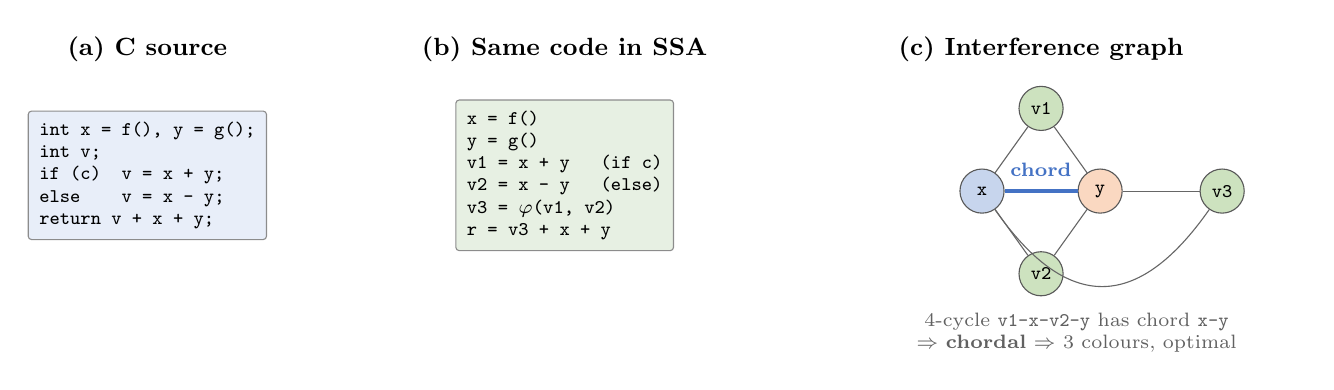
\begin{tikzpicture}[
  code/.style={draw=black!45,rounded corners=1.2pt,fill=lyrIn,align=left,
               inner sep=4pt,font=\scriptsize\ttfamily},
  ig/.style={draw=black!65,circle,inner sep=0pt,minimum size=0.56cm,font=\scriptsize},
  ed/.style={draw=black!60,thin},
  pcap/.style={font=\small\bfseries,align=center},
  ann/.style={font=\scriptsize,color=black!62,align=center}]

%---------------- (a) original C ----------------
\node[pcap] at (0,2.15) {(a) C source};
\node[code] (c1) at (0,0.55)
  {int x = f(), y = g();\\
   int v;\\
   if (c)\ \ v = x + y;\\
   else\ \ \ \ v = x - y;\\
   return v + x + y;};

%---------------- (b) SSA form ----------------
\begin{scope}[xshift=5.3cm]
  \node[pcap] at (0,2.15) {(b) Same code in SSA};
  \node[code,fill=lyrAna] (c2) at (0,0.55)
    {x\ = f()\\
     y\ = g()\\
     v1 = x + y\ \ \ (if c)\\
     v2 = x - y\ \ \ (else)\\
     v3 = $\varphi$(v1, v2)\\
     r\ = v3 + x + y};
\end{scope}

%---------------- (c) interference graph ----------------
\begin{scope}[xshift=10.6cm,yshift=0.35cm]
  \node[pcap] at (0.75,1.80) {(c) Interference graph};
  \node[ig,fill=regA!30] (vx)  at (0,0)        {\texttt{x}};
  \node[ig,fill=regB!30] (vy)  at (1.50,0)     {\texttt{y}};
  \node[ig,fill=regC!35] (v1)  at (0.75,1.05)  {\texttt{v1}};
  \node[ig,fill=regC!35] (v2)  at (0.75,-1.05) {\texttt{v2}};
  \node[ig,fill=regC!35] (v3)  at (3.05,0)     {\texttt{v3}};
  \draw[ed] (vx)--(v1); \draw[ed] (v1)--(vy);
  \draw[ed] (vx)--(v2); \draw[ed] (v2)--(vy);
  \draw[ed] (vy)--(v3);
  \draw[ed] (vx) to[out=-55,in=235,looseness=1.5] (v3);
  \draw[iiitkblue,line width=1.2pt] (vx)--(vy)
        node[midway,above=0.5mm,font=\scriptsize\bfseries,color=iiitkblue]{chord};
  \node[ann,text width=5.6cm] at (1.2,-1.80)
    {4-cycle \texttt{v1-x-v2-y} has chord \texttt{x-y} $\Rightarrow$
     \textbf{chordal} $\Rightarrow$ 3 colours, optimal};
\end{scope}
\end{tikzpicture}
\end{adjustbox}}

%----------------------------------------------------------------------
% 5. FIGURE 2 -- Slide 8: system pipeline, allocator is the swappable box
%----------------------------------------------------------------------
\newcommand{\FigPipeline}{%
\begin{adjustbox}{max width=\textwidth,max totalheight=6.0cm}
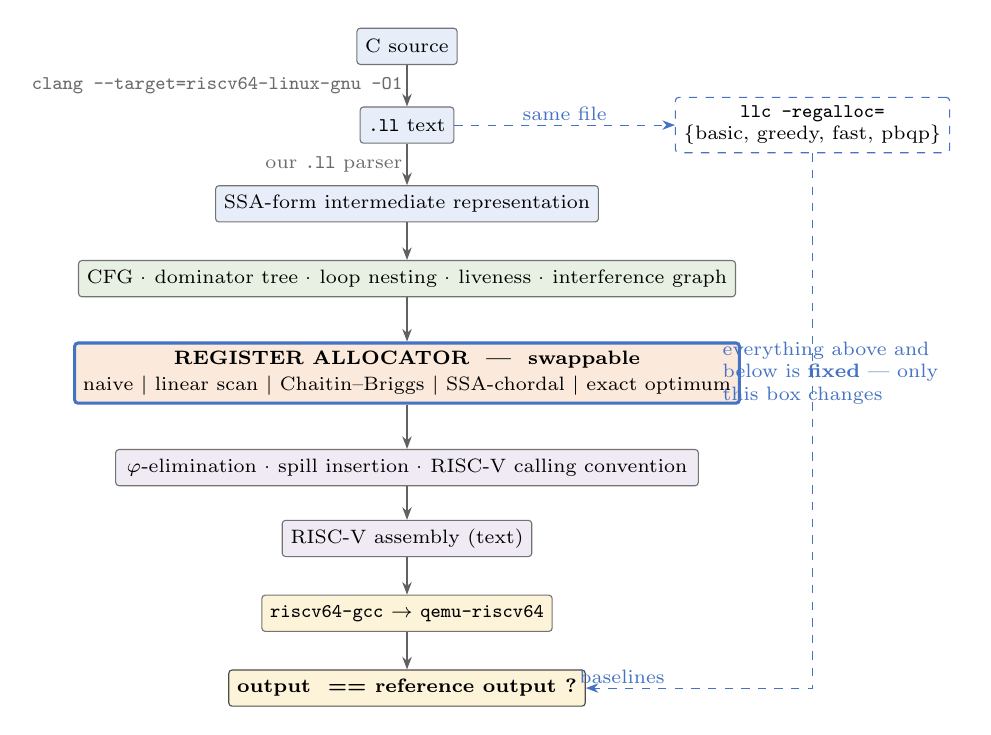
\begin{tikzpicture}[
  n/.style={draw=black!55,rounded corners=1.2pt,align=center,
            font=\scriptsize,inner sep=3pt,minimum height=0.46cm},
  wide/.style={n,minimum width=7.4cm},
  fl/.style={-{Stealth[length=1.6mm]},draw=black!62},
  lbl/.style={font=\scriptsize,color=black!58,inner sep=1.5pt}]

\node[n,fill=lyrIn]   (csrc) at (0, 0.00) {C source};
\node[n,fill=lyrIn]   (llt)  at (0,-1.00) {\texttt{.ll} text};
\node[n,fill=lyrIn]   (ir)   at (0,-2.00) {SSA-form intermediate representation};
\node[wide,fill=lyrAna] (ana) at (0,-2.95)
  {CFG \textperiodcentered\ dominator tree \textperiodcentered\ loop nesting
   \textperiodcentered\ liveness \textperiodcentered\ interference graph};
\node[wide,fill=lyrAlloc,draw=iiitkblue,line width=1.1pt] (alloc) at (0,-4.15)
  {\textbf{REGISTER ALLOCATOR \ --- \ swappable}\\[0.4mm]
   naive \textbar\ linear scan \textbar\ Chaitin--Briggs \textbar\
   SSA-chordal \textbar\ exact optimum};
\node[wide,fill=lyrBack] (back) at (0,-5.35)
  {$\varphi$-elimination \textperiodcentered\ spill insertion
   \textperiodcentered\ RISC-V calling convention};
\node[n,fill=lyrBack] (asm)  at (0,-6.25) {RISC-V assembly (text)};
\node[n,fill=lyrEval] (run)  at (0,-7.20)
  {\texttt{riscv64-gcc} $\rightarrow$ \texttt{qemu-riscv64}};
\node[n,fill=lyrEval,draw=black!70] (chk) at (0,-8.15)
  {\textbf{output \ ==\ reference output ?}};

\draw[fl] (csrc) -- node[lbl,left]{\texttt{clang --target=riscv64-linux-gnu -O1}} (llt);
\draw[fl] (llt)  -- node[lbl,left]{our \texttt{.ll} parser} (ir);
\draw[fl] (ir) -- (ana);
\draw[fl] (ana) -- (alloc);
\draw[fl] (alloc) -- (back);
\draw[fl] (back) -- (asm);
\draw[fl] (asm) -- (run);
\draw[fl] (run) -- (chk);

% fixed above and below: only the boxed allocator changes
\node[lbl,anchor=west,text width=3.0cm,align=left,color=iiitkblue]
     at (3.95,-4.15) {everything above and below is \textbf{fixed} --- only this box changes};

% external baselines off the same .ll
\node[n,fill=white,draw=regA,dashed,align=center] (llc) at (5.15,-1.00)
  {\texttt{llc -regalloc=}\\\{basic, greedy, fast, pbqp\}};
\draw[fl,draw=regA,dashed] (llt) -- node[lbl,above,color=regA]{same file} (llc);
\draw[fl,draw=regA,dashed] (llc) |- node[lbl,pos=0.92,above,color=regA]{baselines} (chk.east);
\end{tikzpicture}
\end{adjustbox}}

%======================================================================
\title{Design and Implementation of an SSA-Based RISC-V Compiler with
       Comparative Register Allocation}
\author{Shaun Alan Joseph \and Rishi Sharma \and Komal \and Aswin Parames}
\institute{Indian Institute of Information Technology Kottayam}
\date{9 September 2026}

\begin{document}

%======================= 1. TITLE =====================================
\begin{frame}
\vspace{0.9cm}
\begin{center}
{\large\textbf{Design and Implementation of an SSA-Based RISC-V Compiler\\[1mm]
 with Comparative Register Allocation}}\\[7mm]
{\footnotesize
\begin{tabular}{@{}c@{\hspace{7mm}}c@{\hspace{7mm}}c@{\hspace{7mm}}c@{}}
Shaun Alan Joseph & Rishi Sharma & Komal & Aswin Parames \\[0.4mm]
{\scriptsize\color{black!60}2023BCD0006} &
{\scriptsize\color{black!60}2023BCD0023} &
{\scriptsize\color{black!60}2023BCD0011} &
{\scriptsize\color{black!60}2023BCD0024} \\
\end{tabular}}\\[4mm]
{\footnotesize\textbf{Guided by:} Dr.\ Nandini J Warrier}\\[2mm]
{\footnotesize Dept.\ of Computer Science and Engineering}\\[1mm]
{\footnotesize Indian Institute of Information Technology, Kottayam}\\[5mm]
{\scriptsize\color{black!55} B.Tech Project \textperiodcentered\ Phase 1
 \textperiodcentered\ Review 1 \textperiodcentered\ 9 September 2026}
\end{center}
\end{frame}

%======================= 2. INTRODUCTION ==============================
\begin{frame}{Introduction: Register Allocation}
\textbf{The last big decision a compiler makes}
\begin{itemize}\small
  \item A program uses unlimited named values. A CPU has few \textbf{registers}
        --- 32 on RISC-V, 16 on x86-64
  \item Values that don't fit are \textbf{spilled} to memory. A spilled value
        costs a load and a store on \emph{every} access --- inside a loop,
        every iteration
  \item One of the highest-impact passes in a compiler backend
  \item \textbf{Chaitin (1981):} build an \textbf{interference graph} --- one
        node per value, an edge between values alive at the same time --- then
        colour it with \emph{k} colours, where \emph{k} = number of registers
\end{itemize}
\end{frame}

%======================= 3. SSA BACKGROUND ============================
\begin{frame}{Background: SSA Form}
\vspace{-1mm}
\begin{columns}[T]
\begin{column}{0.49\textwidth}
{\small\textbf{Static Single Assignment (SSA)}}
\begin{itemize}\scriptsize
  \item Every value assigned \textbf{exactly once}. Reassignment creates a new
        value: \texttt{x1}, \texttt{x2}, \texttt{x3}
  \item Where control flow merges, a \textbf{$\varphi$-function} picks whichever
        value arrived: \texttt{x3 = $\varphi$(x1, x2)}
  \item Used by LLVM, GCC, HotSpot, V8 --- the normal form of modern compilers
\end{itemize}
\end{column}
\begin{column}{0.49\textwidth}
{\small\textbf{Why SSA changes the problem}}
\begin{itemize}\scriptsize
  \item In general interference graphs can be \emph{any} shape, and colouring
        an arbitrary graph is NP-hard --- the textbook reason for heuristics
  \item Interference graphs of SSA programs are always \textbf{chordal}
  \item Chordal graphs colour \textbf{optimally, in linear time}
  \item Established by Hack \& Goos and by Pereira \& Palsberg, both 2005
\end{itemize}
\end{column}
\end{columns}
\vspace{2mm}
\centering\FigChordality
\end{frame}

%======================= 4a. LITERATURE (lines) =======================
\begin{frame}{Literature Survey}
\framesubtitle{Two lines of work}
\vspace{-1mm}
{\footnotesize\textbf{The classical line --- all heuristics, no optimality guarantee}}\par\vspace{1mm}
{\scriptsize
\begin{tabular}{@{}p{3.6cm}p{1.1cm}p{8.2cm}@{}}
\toprule
Work & Year & Contribution \\
\midrule
Chaitin et al.              & 1981 & Interference-graph formulation; showed the problem is NP-hard in general \\
Briggs, Cooper \& Torczon   & 1994 & \textbf{Optimistic colouring.} Ancestor of most production allocators \\
George \& Appel             & 1996 & Iterated coalescing --- removes redundant copy instructions \\
Poletto \& Sarkar           & 1999 & \textbf{Linear scan.} Drops graph colouring for speed; what JITs ship \\
\bottomrule
\end{tabular}}\par\vspace{2.5mm}
{\footnotesize\textbf{The SSA line --- and what it already established}}\par\vspace{1mm}
{\scriptsize
\begin{tabular}{@{}p{3.6cm}p{1.1cm}p{8.2cm}@{}}
\toprule
Work & Year & Contribution \\
\midrule
Tarjan \& Yannakakis          & 1984    & Linear-time chordality test and colouring order \\
\textbf{Hack \& Goos}         & 2005--06& SSA interference graphs are \textbf{chordal} $\Rightarrow$ optimal colouring in linear time \\
\textbf{Pereira \& Palsberg}  & 2005    & Built a chordal allocator, measured 23,681 Java methods. \textbf{$\sim$95\% of graphs are chordal} \\
Bouchez, Darte \& Rastello    & 2006    & The remaining hardness is in \textbf{spilling and coalescing}, not colouring \\
\bottomrule
\end{tabular}}
\end{frame}

%======================= 4b. LITERATURE (their numbers) ===============
\begin{frame}{Literature Survey}
\framesubtitle{Their measured results --- we reproduce these, we don't discover them}
\vspace{2mm}
\centering
{\footnotesize
\begin{tabular}{@{}p{5.4cm}p{7.4cm}@{}}
\toprule
Question & Published answer \emph{(Pereira \& Palsberg, Table 1)} \\
\midrule
Optimal vs.\ classical heuristic?          & \textbf{4.13 vs 4.17} registers/method --- under 1\% \\
Does $\varphi$-elimination destroy chordality? & \textbf{No --- it improves it.} 91\% $\rightarrow$ 95.5\% \\
Does the advantage survive few registers?  & Better at \emph{k}=6, roughly equal at \emph{k}=18 \\
\bottomrule
\end{tabular}}
\vspace{5mm}

\begin{minipage}{0.86\textwidth}\small
\textbf{We are not claiming to discover any of this.} These are the numbers we
expect to reproduce --- on a different processor, in our own compiler --- and
knowing them in advance is how we will tell whether our implementation is
correct.
\end{minipage}
\end{frame}

%======================= 5. MOTIVATION ================================
\begin{frame}{Motivation: Why Build Another One}
{\small\textbf{The algorithms are known. The comparison between them is not reliable.}}\par\vspace{2mm}
{\scriptsize Every published comparison used a different compiler, target and
benchmark set:}\par\vspace{1.5mm}
\centering
{\scriptsize
\begin{tabular}{@{}p{3.4cm}p{2.2cm}p{2.6cm}p{4.0cm}@{}}
\toprule
Work & Compiler & Target & Benchmarks \\
\midrule
Pereira \& Palsberg & JoeQ      & Java bytecode & Java standard library \\
Hack \& Goos        & libFirm   & x86           & SPEC \\
Poletto \& Sarkar   & their own & x86           & their own set \\
LLVM \texttt{greedy}& LLVM      & many          & LLVM's own suite \\
\bottomrule
\end{tabular}}\par\vspace{3mm}
\begin{minipage}{0.92\textwidth}\scriptsize
\textbf{So the numbers can't be placed side by side.} A difference between two
published results might be the algorithm --- or the compiler, the processor, or
the test programs.
\end{minipage}\par\vspace{2.5mm}
\begin{minipage}{0.92\textwidth}
{\small\textbf{What we build instead}}
\begin{itemize}\scriptsize
  \item \textbf{One} compiler, \textbf{one} IR, \textbf{one} benchmark set,
        \textbf{one} backend --- with the allocator as a swappable part
  \item Every difference in output is then caused by the algorithm and nothing else
  \item On \textbf{RISC-V}, where this comparison hasn't been published
\end{itemize}
\end{minipage}
\end{frame}

%======================= 6. PROBLEM STATEMENT =========================
\begin{frame}{Problem Statement}
\vspace{1mm}
\begin{minipage}{0.95\textwidth}
\small\textbf{Design and implement an SSA-based RISC-V compiler in which the
register allocator is a swappable component, implement five allocation
strategies, and compare them under identical conditions.}
\end{minipage}
\vspace{4mm}

{\small\textbf{Three things we measure}}
\begin{itemize}\small
  \item[\textbf{1}] \textbf{Allocation quality.} How many spills does each
        algorithm produce on the same program? Compared against LLVM's
        production allocators, and against a true optimum from an exact solver
        on small functions.
  \item[\textbf{2}] \textbf{Effect of register count.} RISC-V has two official
        integer register configurations --- \textbf{RV32I/RV64I with 32}, and
        \textbf{RV32E with 16}, used in embedded chips. We run every allocator
        on both. Real hardware, not an artificial setting.
  \item[\textbf{3}] \textbf{Cost of the algorithm.} How much work each allocator
        does, counted in operations rather than seconds, so the numbers
        reproduce on any machine.
\end{itemize}
\end{frame}

%======================= 7. SCOPE =====================================
\begin{frame}{Scope of Work}
\vspace{3mm}
\centering
{\footnotesize
\begin{tabular}{@{}p{2.1cm}p{10.6cm}@{}}
\toprule
Layer & Components \\
\midrule
Input      & Textual LLVM IR (\texttt{.ll}) parser, defined subset \\[0.8mm]
Analysis   & CFG \textperiodcentered\ dominator tree \textperiodcentered\ loop detection \textperiodcentered\ liveness \textperiodcentered\ interference graph \textperiodcentered\ chordality test \\[0.8mm]
Allocation & \textbf{Five allocators:} naive \textperiodcentered\ linear scan \textperiodcentered\ Chaitin--Briggs \textperiodcentered\ SSA/chordal \textperiodcentered\ exact optimum \textperiodcentered\ plus coalescing \\[0.8mm]
Backend    & $\varphi$-elimination \textperiodcentered\ spill insertion \textperiodcentered\ RISC-V calling convention \textperiodcentered\ assembly emission \\[0.8mm]
Validation & Static allocation verifier \textperiodcentered\ differential testing \textperiodcentered\ random program testing \\[0.8mm]
Evaluation & Metrics \textperiodcentered\ LLVM \texttt{llc} baselines \textperiodcentered\ 16- vs 32-register comparison \textperiodcentered\ plots \textperiodcentered\ graph visualiser \\
\bottomrule
\end{tabular}}
\vspace{5mm}

\begin{minipage}{0.93\textwidth}\footnotesize
\textbf{Beating LLVM's \texttt{greedy} is not a goal.} Landing within a
constant factor and explaining the gap is.
\end{minipage}
\end{frame}

%======================= 8. ARCHITECTURE ==============================
\begin{frame}{Proposed Architecture}
\vspace{0.5mm}
\centering\FigPipeline
\end{frame}

%======================= 9. FIVE ALLOCATORS ===========================
\begin{frame}{The Five Allocators}
{\scriptsize All five consume \textbf{the same interference graph} and
\textbf{the same register budget}. Any difference in output is caused by the
algorithm alone.}\par\vspace{2mm}
{\scriptsize
\begin{tabular}{@{}p{2.5cm}p{4.6cm}p{5.7cm}@{}}
\toprule
Allocator & What it does & Why it's in the study \\
\midrule
\textbf{Naive}            & Spill everything & Correctness floor. Gets the pipeline working before any real algorithm exists \\
\textbf{Linear scan} (1999)& One pass over live intervals, no graph & Speed baseline --- what JITs ship \\
\textbf{Chaitin--Briggs} (1981/94) & Build $\rightarrow$ simplify $\rightarrow$ optimistic spill $\rightarrow$ select & The classical heuristic. Main comparison point \\
\textbf{SSA / chordal} (2005) & Colour along the order from Maximum Cardinality Search & \textbf{Optimal colouring in linear time}, because SSA graphs are chordal \\
\textbf{Exact optimum}    & Integer linear program, off-the-shelf solver & Too slow for real use; small functions only, gives a \textbf{true reference point} \\
\emph{+ Coalescing} (1996)& Removes redundant copies & Add-on to the graph-based allocators \\
\bottomrule
\end{tabular}}\end{frame}

%======================= 10. EVALUATION ===============================
\begin{frame}{Evaluation and Correctness}
\vspace{-1mm}
\begin{columns}[T]
\begin{column}{0.56\textwidth}
{\scriptsize\textbf{Metrics} --- all counted, never wall-clock}\par\vspace{1mm}
{\scriptsize
\begin{tabular}{@{}p{3.3cm}p{3.6cm}@{}}
\toprule
Metric & What it tells us \\
\midrule
Static spill count & The headline quality number \\
Spills weighted by $10^{\text{loop depth}}$ & Standard proxy for real runtime cost \\
Distance from the exact optimum & How far each heuristic really is from best possible \\
Executed instruction count (QEMU) & End-to-end quality, deterministic \\
Allocator operations executed & Cost side of the quality/cost trade \\
\bottomrule
\end{tabular}}
\end{column}
\begin{column}{0.42\textwidth}
{\scriptsize\textbf{Register-count comparison} --- both are real RISC-V
configurations, not an artificial knob}\par\vspace{1mm}
{\scriptsize
\begin{tabular}{@{}p{2.1cm}p{3.1cm}@{}}
\toprule
Profile & Integer registers \\
\midrule
RV64I / RV32I & 32 \\
\textbf{RV32E} & \textbf{16} --- official embedded profile, high pressure \\
\bottomrule
\end{tabular}}\par\vspace{2mm}
{\scriptsize\textbf{Baselines:} \texttt{llc -regalloc=}\{basic, greedy, fast,
pbqp\} on \textbf{identical IR}}
\end{column}
\end{columns}
\vspace{2.5mm}
\begin{minipage}{0.97\textwidth}
{\scriptsize\textbf{Correctness --- an allocator that miscompiles silently
invalidates every number.} Three independent layers, starting week 1:}
\begin{enumerate}\scriptsize
  \item \textbf{Static verifier} --- checks the allocation without running
        anything: no two simultaneously-alive values share a register, spill
        slots don't overlap
  \item \textbf{Differential testing} --- every benchmark's output compared
        against the \texttt{clang} build of the same source
  \item \textbf{Random program generation} --- auto-generated C programs, output
        compared against GCC
\end{enumerate}
\end{minipage}
\end{frame}

%======================= 11. WORK PLAN ================================
\begin{frame}{Work Plan and Current Status}
\vspace{-1mm}
\begin{columns}[T]
\begin{column}{0.49\textwidth}
{\scriptsize\textbf{Phase 1 --- build the compiler (weeks 1--8)}}\par\vspace{1mm}
{\scriptsize
\begin{tabular}{@{}p{0.8cm}p{5.3cm}@{}}
\toprule
Weeks & Work \\
\midrule
1--2 & Toolchain \textperiodcentered\ end-to-end spike \textperiodcentered\ \texttt{.ll} parser \textperiodcentered\ IR structures \textperiodcentered\ CFG \\
3--4 & Dominator tree \textperiodcentered\ loop detection \textperiodcentered\ liveness \textperiodcentered\ interference graph \textperiodcentered\ naive allocator \\
5--6 & Linear scan \textperiodcentered\ Chaitin--Briggs \\
7--8 & $\varphi$-elimination \textperiodcentered\ RISC-V calling convention \textperiodcentered\ verifier \textperiodcentered\ differential testing \\
\bottomrule
\end{tabular}}
\end{column}
\begin{column}{0.49\textwidth}
{\scriptsize\textbf{Phase 2 --- the comparison (weeks 9--16)}}\par\vspace{1mm}
{\scriptsize
\begin{tabular}{@{}p{0.9cm}p{5.2cm}@{}}
\toprule
Weeks & Work \\
\midrule
9--10  & Benchmarks \textperiodcentered\ LLVM \texttt{llc} baselines \textperiodcentered\ SSA/chordal allocator \\
11--12 & Exact solver on small functions \textperiodcentered\ coalescing \\
13--14 & 16- vs 32-register comparison across all allocators \textperiodcentered\ slack \\
15--16 & Results \textperiodcentered\ visualiser \textperiodcentered\ report \\
\bottomrule
\end{tabular}}
\end{column}
\end{columns}
\vspace{3mm}
{\scriptsize\textbf{Current status}}
\begin{itemize}\scriptsize
  \item Title and scope finalised with the guide
  \item Core literature reviewed, including the specific numbers we expect to reproduce
  \item Architecture and module interfaces specified; work divided across four tracks
  \item \textbf{Toolchain validated end-to-end.} C $\rightarrow$ \texttt{clang}
        $\rightarrow$ RISC-V IR $\rightarrow$ \texttt{llc} $\rightarrow$ assembly
        $\rightarrow$ \texttt{riscv64-linux-gnu-gcc} $\rightarrow$
        \texttt{qemu-riscv64}, output identical to the host-compiled reference
  \item \textbf{All four LLVM baseline allocators confirmed on RISC-V --- and they
        already differentiate.} On a small loop kernel, \texttt{fast} emits
        \textbf{20} stack accesses where \texttt{basic}, \texttt{greedy} and
        \texttt{pbqp} emit \textbf{2}
\end{itemize}
\end{frame}

%======================= 12a. APPLICATIONS ============================
\begin{frame}{Applications}
\vspace{2mm}
\begin{itemize}\small
  \item \textbf{A controlled comparison that doesn't currently exist} --- five
        allocators, one compiler, one benchmark set, one target, so the numbers
        are actually comparable
  \item \textbf{RISC-V embedded toolchains} --- RV32E has only 16 registers.
        That's where allocator choice matters most, and it isn't well
        characterised
  \item \textbf{JIT compilers} --- linear scan is deployed because colouring is
        assumed expensive. On SSA, optimal colouring is linear-time; our
        operation counts are the data needed to revisit that
  \item \textbf{Reusable artefacts} --- a readable implementation of five
        allocators on a common IR (production allocators are effectively
        unreadable), a verification harness, and an interference-graph
        visualiser
\end{itemize}
\end{frame}

%======================= 12b. CONCLUSION ==============================
\begin{frame}{Conclusion}
\vspace{2mm}
\begin{itemize}\small
  \item Register allocation is classically graph colouring, NP-hard in general.
        \textbf{For SSA it isn't} --- optimal colouring is linear-time,
        established 2005
  \item The algorithms are known. \textbf{What's missing is a fair comparison}
        --- every published result comes from a different compiler, target and
        benchmark set
  \item We build an SSA-based RISC-V compiler with a \textbf{swappable}
        allocator, implement five strategies, and compare them on both RISC-V
        register profiles
  \item \textbf{Next phase:} complete the analysis layer and classical
        allocators, reach a correct end-to-end pipeline, begin the comparison
\end{itemize}
\vspace{4mm}
\centering{\small\color{black!55} Thank you --- questions welcome.}
\end{frame}

%======================= 13. REFERENCES ===============================
\begin{frame}{References}
\vspace{1mm}
{\scriptsize
\begin{enumerate}\setlength{\itemsep}{1.1mm}
\item G. J. Chaitin \emph{et al.}, ``Register allocation via coloring,''
      \emph{Computer Languages}, vol.\ 6, no.\ 1, pp.\ 47--57, 1981.
\item P. Briggs, K. D. Cooper, and L. Torczon, ``Improvements to graph coloring
      register allocation,'' \emph{ACM TOPLAS}, vol.\ 16, no.\ 3,
      pp.\ 428--455, 1994.
\item L. George and A. W. Appel, ``Iterated register coalescing,''
      \emph{ACM TOPLAS}, vol.\ 18, no.\ 3, pp.\ 300--324, 1996.
\item M. Poletto and V. Sarkar, ``Linear scan register allocation,''
      \emph{ACM TOPLAS}, vol.\ 21, no.\ 5, pp.\ 895--913, 1999.
\item S. Hack and G. Goos, ``Optimal register allocation for SSA-form programs
      in polynomial time,'' \emph{Inf.\ Process.\ Lett.}, vol.\ 98, no.\ 4,
      pp.\ 150--155, 2006.
\item F. M. Q. Pereira and J. Palsberg, ``Register allocation via coloring of
      chordal graphs,'' in \emph{Proc.\ APLAS}, 2005, pp.\ 315--329.
\item F. Bouchez, A. Darte, and F. Rastello, ``Register allocation: What does
      the NP-completeness proof of Chaitin et al.\ really prove?,'' in
      \emph{Proc.\ LCPC}, 2006, pp.\ 283--298.
\item R. E. Tarjan and M. Yannakakis, ``Simple linear-time algorithms to test
      chordality of graphs\dots,'' \emph{SIAM J.\ Comput.}, vol.\ 13, no.\ 3,
      pp.\ 566--579, 1984.
\item R. Casta\~{n}eda Lozano and C. Schulte, ``Survey on combinatorial register
      allocation and instruction scheduling,'' \emph{ACM Comput.\ Surv.},
      vol.\ 52, no.\ 3, 2019.
\end{enumerate}}
\end{frame}

\end{document}
